% Options for packages loaded elsewhere
\PassOptionsToPackage{unicode}{hyperref}
\PassOptionsToPackage{hyphens}{url}
%
\documentclass[
]{article}
\usepackage{amsmath,amssymb}
\usepackage{lmodern}
\usepackage{iftex}
\ifPDFTeX
  \usepackage[T1]{fontenc}
  \usepackage[utf8]{inputenc}
  \usepackage{textcomp} % provide euro and other symbols
\else % if luatex or xetex
  \usepackage{unicode-math}
  \defaultfontfeatures{Scale=MatchLowercase}
  \defaultfontfeatures[\rmfamily]{Ligatures=TeX,Scale=1}
\fi
% Use upquote if available, for straight quotes in verbatim environments
\IfFileExists{upquote.sty}{\usepackage{upquote}}{}
\IfFileExists{microtype.sty}{% use microtype if available
  \usepackage[]{microtype}
  \UseMicrotypeSet[protrusion]{basicmath} % disable protrusion for tt fonts
}{}
\makeatletter
\@ifundefined{KOMAClassName}{% if non-KOMA class
  \IfFileExists{parskip.sty}{%
    \usepackage{parskip}
  }{% else
    \setlength{\parindent}{0pt}
    \setlength{\parskip}{6pt plus 2pt minus 1pt}}
}{% if KOMA class
  \KOMAoptions{parskip=half}}
\makeatother
\usepackage{xcolor}
\usepackage[margin=1in]{geometry}
\usepackage{color}
\usepackage{fancyvrb}
\newcommand{\VerbBar}{|}
\newcommand{\VERB}{\Verb[commandchars=\\\{\}]}
\DefineVerbatimEnvironment{Highlighting}{Verbatim}{commandchars=\\\{\}}
% Add ',fontsize=\small' for more characters per line
\usepackage{framed}
\definecolor{shadecolor}{RGB}{248,248,248}
\newenvironment{Shaded}{\begin{snugshade}}{\end{snugshade}}
\newcommand{\AlertTok}[1]{\textcolor[rgb]{0.94,0.16,0.16}{#1}}
\newcommand{\AnnotationTok}[1]{\textcolor[rgb]{0.56,0.35,0.01}{\textbf{\textit{#1}}}}
\newcommand{\AttributeTok}[1]{\textcolor[rgb]{0.77,0.63,0.00}{#1}}
\newcommand{\BaseNTok}[1]{\textcolor[rgb]{0.00,0.00,0.81}{#1}}
\newcommand{\BuiltInTok}[1]{#1}
\newcommand{\CharTok}[1]{\textcolor[rgb]{0.31,0.60,0.02}{#1}}
\newcommand{\CommentTok}[1]{\textcolor[rgb]{0.56,0.35,0.01}{\textit{#1}}}
\newcommand{\CommentVarTok}[1]{\textcolor[rgb]{0.56,0.35,0.01}{\textbf{\textit{#1}}}}
\newcommand{\ConstantTok}[1]{\textcolor[rgb]{0.00,0.00,0.00}{#1}}
\newcommand{\ControlFlowTok}[1]{\textcolor[rgb]{0.13,0.29,0.53}{\textbf{#1}}}
\newcommand{\DataTypeTok}[1]{\textcolor[rgb]{0.13,0.29,0.53}{#1}}
\newcommand{\DecValTok}[1]{\textcolor[rgb]{0.00,0.00,0.81}{#1}}
\newcommand{\DocumentationTok}[1]{\textcolor[rgb]{0.56,0.35,0.01}{\textbf{\textit{#1}}}}
\newcommand{\ErrorTok}[1]{\textcolor[rgb]{0.64,0.00,0.00}{\textbf{#1}}}
\newcommand{\ExtensionTok}[1]{#1}
\newcommand{\FloatTok}[1]{\textcolor[rgb]{0.00,0.00,0.81}{#1}}
\newcommand{\FunctionTok}[1]{\textcolor[rgb]{0.00,0.00,0.00}{#1}}
\newcommand{\ImportTok}[1]{#1}
\newcommand{\InformationTok}[1]{\textcolor[rgb]{0.56,0.35,0.01}{\textbf{\textit{#1}}}}
\newcommand{\KeywordTok}[1]{\textcolor[rgb]{0.13,0.29,0.53}{\textbf{#1}}}
\newcommand{\NormalTok}[1]{#1}
\newcommand{\OperatorTok}[1]{\textcolor[rgb]{0.81,0.36,0.00}{\textbf{#1}}}
\newcommand{\OtherTok}[1]{\textcolor[rgb]{0.56,0.35,0.01}{#1}}
\newcommand{\PreprocessorTok}[1]{\textcolor[rgb]{0.56,0.35,0.01}{\textit{#1}}}
\newcommand{\RegionMarkerTok}[1]{#1}
\newcommand{\SpecialCharTok}[1]{\textcolor[rgb]{0.00,0.00,0.00}{#1}}
\newcommand{\SpecialStringTok}[1]{\textcolor[rgb]{0.31,0.60,0.02}{#1}}
\newcommand{\StringTok}[1]{\textcolor[rgb]{0.31,0.60,0.02}{#1}}
\newcommand{\VariableTok}[1]{\textcolor[rgb]{0.00,0.00,0.00}{#1}}
\newcommand{\VerbatimStringTok}[1]{\textcolor[rgb]{0.31,0.60,0.02}{#1}}
\newcommand{\WarningTok}[1]{\textcolor[rgb]{0.56,0.35,0.01}{\textbf{\textit{#1}}}}
\usepackage{graphicx}
\makeatletter
\def\maxwidth{\ifdim\Gin@nat@width>\linewidth\linewidth\else\Gin@nat@width\fi}
\def\maxheight{\ifdim\Gin@nat@height>\textheight\textheight\else\Gin@nat@height\fi}
\makeatother
% Scale images if necessary, so that they will not overflow the page
% margins by default, and it is still possible to overwrite the defaults
% using explicit options in \includegraphics[width, height, ...]{}
\setkeys{Gin}{width=\maxwidth,height=\maxheight,keepaspectratio}
% Set default figure placement to htbp
\makeatletter
\def\fps@figure{htbp}
\makeatother
\setlength{\emergencystretch}{3em} % prevent overfull lines
\providecommand{\tightlist}{%
  \setlength{\itemsep}{0pt}\setlength{\parskip}{0pt}}
\setcounter{secnumdepth}{-\maxdimen} % remove section numbering
\usepackage{float}
\ifLuaTeX
  \usepackage{selnolig}  % disable illegal ligatures
\fi
\IfFileExists{bookmark.sty}{\usepackage{bookmark}}{\usepackage{hyperref}}
\IfFileExists{xurl.sty}{\usepackage{xurl}}{} % add URL line breaks if available
\urlstyle{same} % disable monospaced font for URLs
\hypersetup{
  pdftitle={Project Part 1},
  pdfauthor={Virginia Brame, Clay Harris, Hai Liu},
  hidelinks,
  pdfcreator={LaTeX via pandoc}}

\title{Project Part 1}
\author{Virginia Brame, Clay Harris, Hai Liu}
\date{2025-02-25}

\begin{document}
\maketitle

\begin{Shaded}
\begin{Highlighting}[]
\NormalTok{knitr}\SpecialCharTok{::}\NormalTok{opts\_chunk}\SpecialCharTok{$}\FunctionTok{set}\NormalTok{(}\AttributeTok{echo=}\ConstantTok{TRUE}\NormalTok{)}
\NormalTok{knitr}\SpecialCharTok{::}\NormalTok{opts\_chunk}\SpecialCharTok{$}\FunctionTok{set}\NormalTok{(}\AttributeTok{cache=}\ConstantTok{TRUE}\NormalTok{, }\AttributeTok{autodep=}\ConstantTok{TRUE}\NormalTok{)}
\NormalTok{knitr}\SpecialCharTok{::}\NormalTok{opts\_chunk}\SpecialCharTok{$}\FunctionTok{set}\NormalTok{(}\AttributeTok{fig.align=}\StringTok{"center"}\NormalTok{, }\AttributeTok{fig.pos=}\StringTok{"H"}\NormalTok{)}
\end{Highlighting}
\end{Shaded}

\hypertarget{data-loading-wrangling-eda}{%
\subsection{Data (loading, wrangling,
EDA)}\label{data-loading-wrangling-eda}}

\begin{Shaded}
\begin{Highlighting}[]
\FunctionTok{library}\NormalTok{(doParallel)}
\NormalTok{cl }\OtherTok{\textless{}{-}} \FunctionTok{makePSOCKcluster}\NormalTok{(parallel}\SpecialCharTok{::}\FunctionTok{detectCores}\NormalTok{(}\AttributeTok{logical =} \ConstantTok{FALSE}\NormalTok{))}
\FunctionTok{registerDoParallel}\NormalTok{(cl)}
\end{Highlighting}
\end{Shaded}

\begin{Shaded}
\begin{Highlighting}[]
\FunctionTok{library}\NormalTok{(tidyverse)}
\FunctionTok{library}\NormalTok{(tidymodels)}
\FunctionTok{library}\NormalTok{(discrim)}
\FunctionTok{library}\NormalTok{(leaflet)}
\FunctionTok{library}\NormalTok{(terra)}
\FunctionTok{library}\NormalTok{(htmlwidgets)}
\FunctionTok{library}\NormalTok{(leafem)}
\FunctionTok{library}\NormalTok{(colordistance)}
\FunctionTok{library}\NormalTok{(jpeg)}
\FunctionTok{library}\NormalTok{(patchwork)}
\FunctionTok{library}\NormalTok{(probably)}
\FunctionTok{library}\NormalTok{(gridExtra)}
\FunctionTok{library}\NormalTok{(plotly)}
\FunctionTok{library}\NormalTok{(mapview)}
\end{Highlighting}
\end{Shaded}

\hypertarget{data-loading-and-wrangling}{%
\subsubsection{Data loading and
wrangling}\label{data-loading-and-wrangling}}

Since we are only interested in the level of ``Blue Tarp'', I create a
new variable \texttt{BT} with only two classes, i.e., ``TRUE'' for
``Blue Tarp'' and ``FALSE'' for everything else.

\begin{Shaded}
\begin{Highlighting}[]
\NormalTok{col\_names }\OtherTok{\textless{}{-}} \FunctionTok{c}\NormalTok{(}\StringTok{\textquotesingle{}ID\textquotesingle{}}\NormalTok{,}\StringTok{\textquotesingle{}X\textquotesingle{}}\NormalTok{,}\StringTok{\textquotesingle{}Y\textquotesingle{}}\NormalTok{,}\StringTok{\textquotesingle{}Map X\textquotesingle{}}\NormalTok{,}\StringTok{\textquotesingle{}Map Y\textquotesingle{}}\NormalTok{,}\StringTok{\textquotesingle{}Lat\textquotesingle{}}\NormalTok{,}\StringTok{\textquotesingle{}Lon\textquotesingle{}}\NormalTok{,}\StringTok{\textquotesingle{}Red\textquotesingle{}}\NormalTok{,}\StringTok{\textquotesingle{}Green\textquotesingle{}}\NormalTok{,}\StringTok{\textquotesingle{}Blue\textquotesingle{}}\NormalTok{)}

\NormalTok{blue\_files }\OtherTok{\textless{}{-}} \FunctionTok{c}\NormalTok{(}
  \StringTok{"orthovnir069\_ROI\_Blue\_Tarps.txt"}\NormalTok{,}
  \StringTok{"orthovnir067\_ROI\_Blue\_Tarps.txt"}\NormalTok{,}
  \StringTok{"orthovnir078\_ROI\_Blue\_Tarps.txt"}
\NormalTok{)}

\NormalTok{non\_blue\_files }\OtherTok{\textless{}{-}} \FunctionTok{c}\NormalTok{(}
  \StringTok{"orthovnir057\_ROI\_NON\_Blue\_Tarps.txt"}\NormalTok{,}
  \StringTok{"orthovnir078\_ROI\_NON\_Blue\_Tarps.txt"}\NormalTok{,}
  \StringTok{"orthovnir067\_ROI\_NOT\_Blue\_Tarps.txt"}\NormalTok{,}
  \StringTok{"orthovnir069\_ROI\_NOT\_Blue\_Tarps.txt"}
\NormalTok{)}

\NormalTok{blue\_data }\OtherTok{\textless{}{-}} \FunctionTok{map\_dfr}\NormalTok{(blue\_files, }\SpecialCharTok{\textasciitilde{}} 
  \FunctionTok{read\_table}\NormalTok{(.x, }\AttributeTok{comment =} \StringTok{";"}\NormalTok{, }\AttributeTok{col\_names =}\NormalTok{ col\_names) }\SpecialCharTok{\%\textgreater{}\%} 
    \FunctionTok{select}\NormalTok{(Lat, Lon, Red, Green, Blue) }\SpecialCharTok{\%\textgreater{}\%} 
    \FunctionTok{mutate}\NormalTok{(}\AttributeTok{BT =} \StringTok{"TRUE"}\NormalTok{)}
\NormalTok{)}

\NormalTok{non\_blue\_data }\OtherTok{\textless{}{-}} \FunctionTok{map\_dfr}\NormalTok{(non\_blue\_files, }\SpecialCharTok{\textasciitilde{}} 
  \FunctionTok{read\_table}\NormalTok{(.x, }\AttributeTok{comment =} \StringTok{";"}\NormalTok{, }\AttributeTok{col\_names =}\NormalTok{ col\_names) }\SpecialCharTok{\%\textgreater{}\%} 
    \FunctionTok{select}\NormalTok{(Lat, Lon, Red, Green, Blue) }\SpecialCharTok{\%\textgreater{}\%} 
    \FunctionTok{mutate}\NormalTok{(}\AttributeTok{BT =} \StringTok{"FALSE"}\NormalTok{)}
\NormalTok{)}

\NormalTok{holdout\_data }\OtherTok{\textless{}{-}} \FunctionTok{bind\_rows}\NormalTok{(blue\_data, non\_blue\_data) }\SpecialCharTok{\%\textgreater{}\%} 
  \FunctionTok{mutate}\NormalTok{(}\AttributeTok{BT =} \FunctionTok{factor}\NormalTok{(BT, }\AttributeTok{levels =} \FunctionTok{c}\NormalTok{(}\StringTok{"TRUE"}\NormalTok{, }\StringTok{"FALSE"}\NormalTok{)))}
\end{Highlighting}
\end{Shaded}

\begin{Shaded}
\begin{Highlighting}[]
\NormalTok{train\_data }\OtherTok{\textless{}{-}} \FunctionTok{read\_csv}\NormalTok{(}\StringTok{"HaitiPixels.csv"}\NormalTok{) }\SpecialCharTok{\%\textgreater{}\%}
  \FunctionTok{mutate}\NormalTok{(}\AttributeTok{BT =} \FunctionTok{factor}\NormalTok{(}\FunctionTok{if\_else}\NormalTok{(Class }\SpecialCharTok{==} \StringTok{"Blue Tarp"}\NormalTok{, }\StringTok{"TRUE"}\NormalTok{, }\StringTok{"FALSE"}\NormalTok{), }\AttributeTok{levels =} \FunctionTok{c}\NormalTok{(}\StringTok{"TRUE"}\NormalTok{, }\StringTok{"FALSE"}\NormalTok{))) }\SpecialCharTok{\%\textgreater{}\%}
  \FunctionTok{select}\NormalTok{(Red, Green, Blue, BT)}
\end{Highlighting}
\end{Shaded}

\hypertarget{eda}{%
\subsubsection{EDA}\label{eda}}

\begin{Shaded}
\begin{Highlighting}[]
\CommentTok{\# Convert}
\NormalTok{holdout\_data\_sp }\OtherTok{\textless{}{-}}\NormalTok{ holdout\_data }\SpecialCharTok{\%\textgreater{}\%} 
  \FunctionTok{rename}\NormalTok{(}\AttributeTok{x =}\NormalTok{ Lon, }\AttributeTok{y =}\NormalTok{ Lat)}
\NormalTok{v }\OtherTok{\textless{}{-}}\NormalTok{ terra}\SpecialCharTok{::}\FunctionTok{vect}\NormalTok{(holdout\_data\_sp, }\AttributeTok{geom =} \FunctionTok{c}\NormalTok{(}\StringTok{"x"}\NormalTok{, }\StringTok{"y"}\NormalTok{), }\AttributeTok{crs =} \StringTok{"EPSG:4326"}\NormalTok{)}

\CommentTok{\# Reproject to UTM (meters)}
\NormalTok{v\_utm }\OtherTok{\textless{}{-}}\NormalTok{ terra}\SpecialCharTok{::}\FunctionTok{project}\NormalTok{(v, }\StringTok{"EPSG:32618"}\NormalTok{)}

\CommentTok{\# Create an empty raster}
\NormalTok{r\_empty }\OtherTok{\textless{}{-}}\NormalTok{ terra}\SpecialCharTok{::}\FunctionTok{rast}\NormalTok{(terra}\SpecialCharTok{::}\FunctionTok{ext}\NormalTok{(v\_utm), }\AttributeTok{resolution =} \FloatTok{0.5}\NormalTok{, }\AttributeTok{crs =} \StringTok{"EPSG:32618"}\NormalTok{)}

\CommentTok{\# Rasterize}
\NormalTok{r\_b1 }\OtherTok{\textless{}{-}}\NormalTok{ terra}\SpecialCharTok{::}\FunctionTok{rasterize}\NormalTok{(v\_utm, r\_empty, }\AttributeTok{field =} \StringTok{"Red"}\NormalTok{, }\AttributeTok{overwrite =} \ConstantTok{TRUE}\NormalTok{)}
\NormalTok{r\_b2 }\OtherTok{\textless{}{-}}\NormalTok{ terra}\SpecialCharTok{::}\FunctionTok{rasterize}\NormalTok{(v\_utm, r\_empty, }\AttributeTok{field =} \StringTok{"Green"}\NormalTok{, }\AttributeTok{overwrite =} \ConstantTok{TRUE}\NormalTok{)}
\NormalTok{r\_b3 }\OtherTok{\textless{}{-}}\NormalTok{ terra}\SpecialCharTok{::}\FunctionTok{rasterize}\NormalTok{(v\_utm, r\_empty, }\AttributeTok{field =} \StringTok{"Blue"}\NormalTok{, }\AttributeTok{overwrite =} \ConstantTok{TRUE}\NormalTok{)}

\CommentTok{\# Combine}
\NormalTok{rgb\_raster }\OtherTok{\textless{}{-}} \FunctionTok{c}\NormalTok{(r\_b1, r\_b2, r\_b3)}

\CommentTok{\# Reproject}
\NormalTok{rgb\_raster\_wgs }\OtherTok{\textless{}{-}}\NormalTok{ terra}\SpecialCharTok{::}\FunctionTok{project}\NormalTok{(rgb\_raster, }\StringTok{"EPSG:4326"}\NormalTok{, }\AttributeTok{overwrite =} \ConstantTok{TRUE}\NormalTok{)}

\CommentTok{\# Convert to brick for leaflet}
\NormalTok{rgb\_brick }\OtherTok{\textless{}{-}}\NormalTok{ raster}\SpecialCharTok{::}\FunctionTok{brick}\NormalTok{(rgb\_raster\_wgs)}
\end{Highlighting}
\end{Shaded}

\begin{Shaded}
\begin{Highlighting}[]
\CommentTok{\# Create map}
\NormalTok{m }\OtherTok{\textless{}{-}} \FunctionTok{leaflet}\NormalTok{(}\AttributeTok{options =} \FunctionTok{leafletOptions}\NormalTok{(}\AttributeTok{maxZoom =} \DecValTok{25}\NormalTok{)) }\SpecialCharTok{\%\textgreater{}\%}
  \FunctionTok{addTiles}\NormalTok{(}\AttributeTok{options =} \FunctionTok{tileOptions}\NormalTok{(}\AttributeTok{maxZoom =} \DecValTok{25}\NormalTok{)) }\SpecialCharTok{\%\textgreater{}\%}
\NormalTok{  leafem}\SpecialCharTok{::}\FunctionTok{addRasterRGB}\NormalTok{(rgb\_brick, }\AttributeTok{r =} \DecValTok{1}\NormalTok{, }\AttributeTok{g =} \DecValTok{2}\NormalTok{, }\AttributeTok{b =} \DecValTok{3}\NormalTok{)}

\ControlFlowTok{if}\NormalTok{ (knitr}\SpecialCharTok{::}\FunctionTok{is\_html\_output}\NormalTok{()) \{}
\NormalTok{  htmlwidgets}\SpecialCharTok{::}\FunctionTok{saveWidget}\NormalTok{(m, }\StringTok{"interactive\_map.html"}\NormalTok{)}
\NormalTok{  htmltools}\SpecialCharTok{::}\FunctionTok{includeHTML}\NormalTok{(}\StringTok{"interactive\_map.html"}\NormalTok{)}
\NormalTok{\} }\ControlFlowTok{else}\NormalTok{ \{}
  \CommentTok{\# Save a static image for PDF output}
  \FunctionTok{mapshot}\NormalTok{(m, }\AttributeTok{file =} \StringTok{"map\_static.png"}\NormalTok{)}
\NormalTok{  knitr}\SpecialCharTok{::}\FunctionTok{include\_graphics}\NormalTok{(}\StringTok{"map\_static.png"}\NormalTok{)}
\NormalTok{\}}
\end{Highlighting}
\end{Shaded}

\begin{center}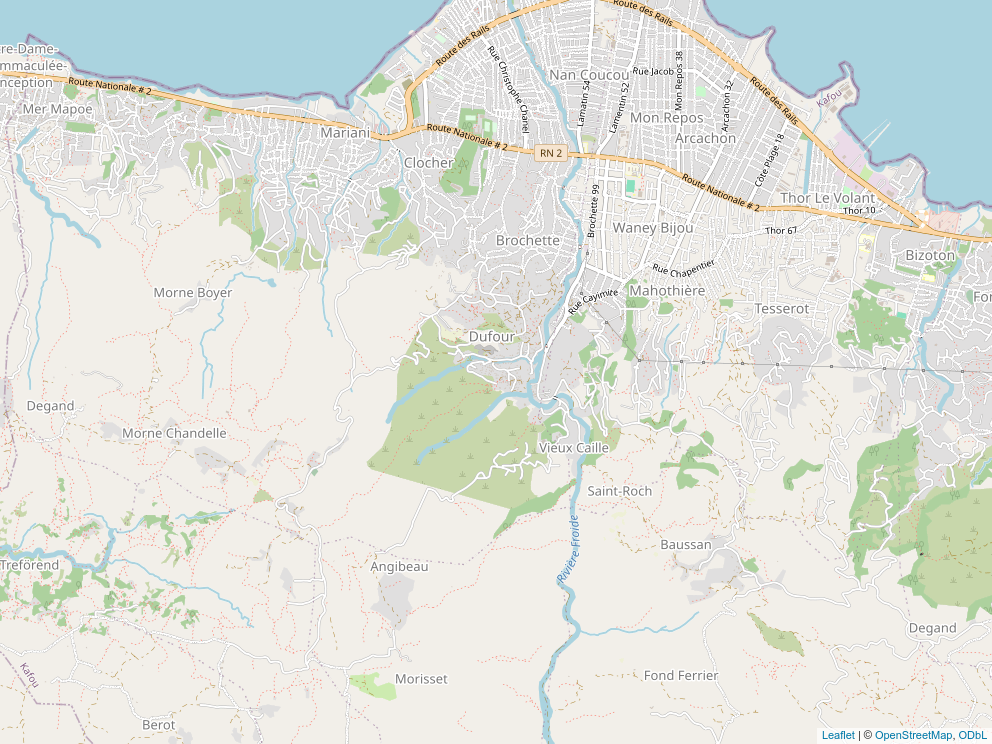
\includegraphics[width=13.78in]{map_static} \end{center}

\begin{Shaded}
\begin{Highlighting}[]
\CommentTok{\# Identify non{-}null pixels}
\NormalTok{non\_na\_mask }\OtherTok{\textless{}{-}} \SpecialCharTok{!}\FunctionTok{is.na}\NormalTok{(r\_b1) }\SpecialCharTok{|} \SpecialCharTok{!}\FunctionTok{is.na}\NormalTok{(r\_b2) }\SpecialCharTok{|} \SpecialCharTok{!}\FunctionTok{is.na}\NormalTok{(r\_b3)}

\CommentTok{\# Count cells}
\NormalTok{non\_na\_cells }\OtherTok{\textless{}{-}} \FunctionTok{sum}\NormalTok{(terra}\SpecialCharTok{::}\FunctionTok{values}\NormalTok{(non\_na\_mask), }\AttributeTok{na.rm =} \ConstantTok{TRUE}\NormalTok{)}

\CommentTok{\# Area of one pixel}
\NormalTok{cell\_area\_km2 }\OtherTok{\textless{}{-}}\NormalTok{ (terra}\SpecialCharTok{::}\FunctionTok{res}\NormalTok{(r\_empty)[}\DecValTok{1}\NormalTok{] }\SpecialCharTok{*}\NormalTok{ terra}\SpecialCharTok{::}\FunctionTok{res}\NormalTok{(r\_empty)[}\DecValTok{2}\NormalTok{]) }\SpecialCharTok{/} \FloatTok{1e6}

\CommentTok{\# Total area}
\NormalTok{total\_area\_km2 }\OtherTok{\textless{}{-}}\NormalTok{ non\_na\_cells }\SpecialCharTok{*}\NormalTok{ cell\_area\_km2}

\CommentTok{\# Print the result}
\NormalTok{total\_area\_km2}
\end{Highlighting}
\end{Shaded}

\begin{verbatim}
## [1] 0.01344958
\end{verbatim}

\begin{Shaded}
\begin{Highlighting}[]
\NormalTok{rgb1 }\OtherTok{\textless{}{-}}\NormalTok{ train\_data }\SpecialCharTok{\%\textgreater{}\%} 
  \FunctionTok{ggplot}\NormalTok{(}\FunctionTok{aes}\NormalTok{(}\AttributeTok{x=}\NormalTok{Red, }\AttributeTok{fill=}\NormalTok{BT))}\SpecialCharTok{+}
  \FunctionTok{geom\_density}\NormalTok{(}\AttributeTok{alpha =} \FloatTok{0.5}\NormalTok{)}
\NormalTok{rgb2 }\OtherTok{\textless{}{-}}\NormalTok{ train\_data }\SpecialCharTok{\%\textgreater{}\%} 
  \FunctionTok{ggplot}\NormalTok{(}\FunctionTok{aes}\NormalTok{(}\AttributeTok{x=}\NormalTok{Green, }\AttributeTok{fill=}\NormalTok{BT))}\SpecialCharTok{+}
  \FunctionTok{geom\_density}\NormalTok{(}\AttributeTok{alpha =} \FloatTok{0.5}\NormalTok{)}
\NormalTok{rgb3 }\OtherTok{\textless{}{-}}\NormalTok{ train\_data }\SpecialCharTok{\%\textgreater{}\%} 
  \FunctionTok{ggplot}\NormalTok{(}\FunctionTok{aes}\NormalTok{(}\AttributeTok{x=}\NormalTok{Blue, }\AttributeTok{fill=}\NormalTok{BT))}\SpecialCharTok{+}
  \FunctionTok{geom\_density}\NormalTok{(}\AttributeTok{alpha =} \FloatTok{0.5}\NormalTok{)}

\FunctionTok{grid.arrange}\NormalTok{(rgb1, rgb2, rgb3)}
\end{Highlighting}
\end{Shaded}

\begin{center}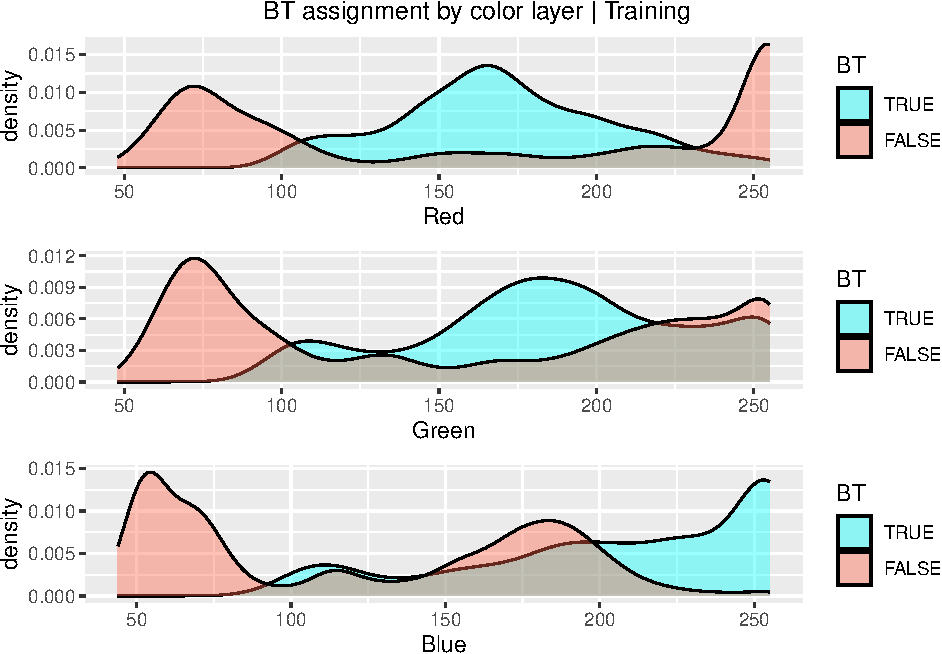
\includegraphics{ProjectPart1_MERGED_files/figure-latex/density plots-1} \end{center}

Understanding that: - Blue is 0,0,255 - Green is 0,255,0 - Red is
255,0,0

\begin{Shaded}
\begin{Highlighting}[]
\FunctionTok{plot\_ly}\NormalTok{(train\_data, }\AttributeTok{x =} \SpecialCharTok{\textasciitilde{}}\NormalTok{Red, }\AttributeTok{y =} \SpecialCharTok{\textasciitilde{}}\NormalTok{Green, }\AttributeTok{z =} \SpecialCharTok{\textasciitilde{}}\NormalTok{Blue, }\AttributeTok{color =} \SpecialCharTok{\textasciitilde{}}\NormalTok{BT, }
        \AttributeTok{colors =} \FunctionTok{c}\NormalTok{(}\StringTok{"orange"}\NormalTok{, }\StringTok{"lightblue"}\NormalTok{)) }\SpecialCharTok{\%\textgreater{}\%}
  \FunctionTok{add\_markers}\NormalTok{() }\SpecialCharTok{\%\textgreater{}\%}
  \FunctionTok{layout}\NormalTok{(}\AttributeTok{title =} \StringTok{"Test Data | 3D RGB Plot by BlueTarp"}\NormalTok{,}
         \AttributeTok{scene =} \FunctionTok{list}\NormalTok{(}\AttributeTok{xaxis =} \FunctionTok{list}\NormalTok{(}\AttributeTok{title =} \StringTok{\textquotesingle{}Red\textquotesingle{}}\NormalTok{),}
                      \AttributeTok{yaxis =} \FunctionTok{list}\NormalTok{(}\AttributeTok{title =} \StringTok{\textquotesingle{}Green\textquotesingle{}}\NormalTok{),}
                      \AttributeTok{zaxis =} \FunctionTok{list}\NormalTok{(}\AttributeTok{title =} \StringTok{\textquotesingle{}Blue\textquotesingle{}}\NormalTok{)))}
\end{Highlighting}
\end{Shaded}

\begin{center}
\includegraphics{ProjectPart1_MERGED_files/figure-latex/plotly plot-1} \end{center}

Here we can clearly see the separation of the two levels of BlueTarp in
the training data.

\begin{Shaded}
\begin{Highlighting}[]
\NormalTok{image\_path }\OtherTok{\textless{}{-}} \StringTok{"orthovnir078\_makeshift\_villiage1.jpg"}
\NormalTok{colordistance}\SpecialCharTok{::}\FunctionTok{plotPixels}\NormalTok{(image\_path)}
\end{Highlighting}
\end{Shaded}

\begin{center}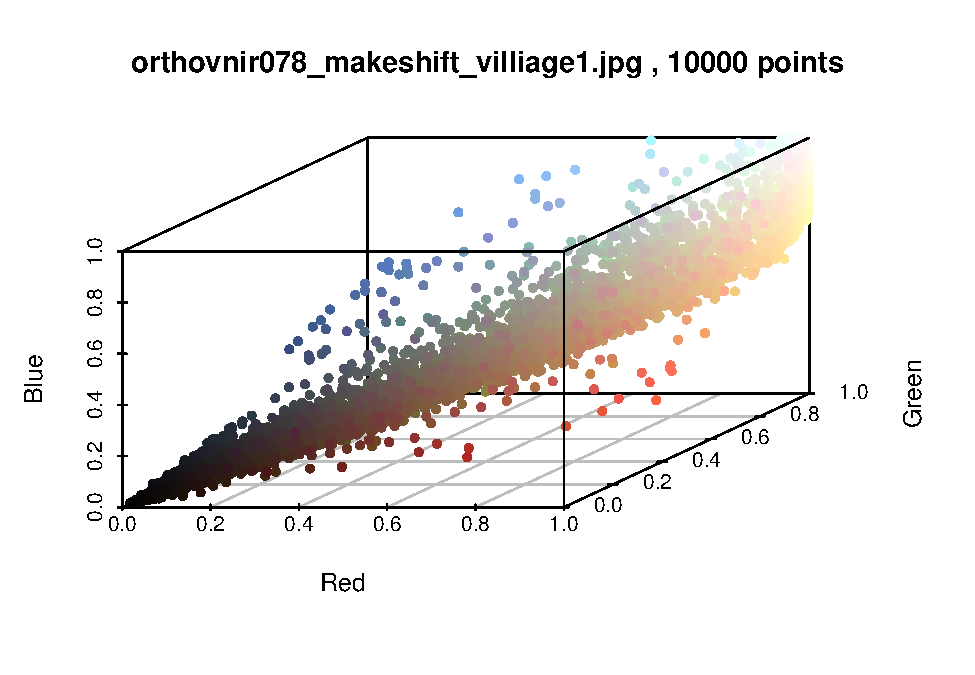
\includegraphics{ProjectPart1_MERGED_files/figure-latex/makeshift village-1} \end{center}

\begin{Shaded}
\begin{Highlighting}[]
\NormalTok{H8hist }\OtherTok{\textless{}{-}}\NormalTok{ colordistance}\SpecialCharTok{::}\FunctionTok{getImageHist}\NormalTok{(image\_path, }\AttributeTok{bins=}\FunctionTok{c}\NormalTok{(}\DecValTok{1}\NormalTok{, }\DecValTok{1}\NormalTok{, }\DecValTok{2}\NormalTok{))}
\end{Highlighting}
\end{Shaded}

\begin{center}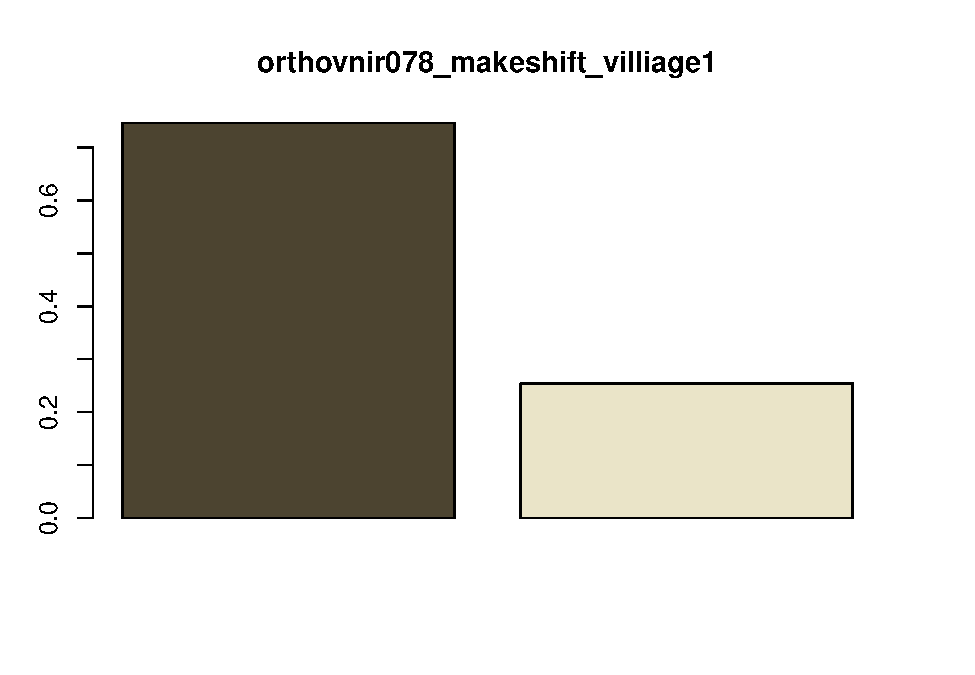
\includegraphics{ProjectPart1_MERGED_files/figure-latex/makeshift village-2} \end{center}

\begin{Shaded}
\begin{Highlighting}[]
\CommentTok{\# Number of pixels}
\NormalTok{n }\OtherTok{\textless{}{-}} \FunctionTok{nrow}\NormalTok{(holdout\_data)}
\NormalTok{maxHeight }\OtherTok{\textless{}{-}} \DecValTok{65500}
\NormalTok{height }\OtherTok{\textless{}{-}} \FunctionTok{min}\NormalTok{(n, maxHeight)}
\NormalTok{width }\OtherTok{\textless{}{-}} \FunctionTok{ceiling}\NormalTok{(n }\SpecialCharTok{/}\NormalTok{ height)}
\NormalTok{total\_pixels }\OtherTok{\textless{}{-}}\NormalTok{ height }\SpecialCharTok{*}\NormalTok{ width}

\CommentTok{\# Normalize RGB}
\NormalTok{r }\OtherTok{\textless{}{-}}\NormalTok{ holdout\_data}\SpecialCharTok{$}\NormalTok{Red }\SpecialCharTok{/} \DecValTok{255}
\NormalTok{g }\OtherTok{\textless{}{-}}\NormalTok{ holdout\_data}\SpecialCharTok{$}\NormalTok{Green }\SpecialCharTok{/} \DecValTok{255}
\NormalTok{b }\OtherTok{\textless{}{-}}\NormalTok{ holdout\_data}\SpecialCharTok{$}\NormalTok{Blue }\SpecialCharTok{/} \DecValTok{255}

\CommentTok{\# Calculate padding}
\NormalTok{pad }\OtherTok{\textless{}{-}}\NormalTok{ total\_pixels }\SpecialCharTok{{-}}\NormalTok{ n}

\CommentTok{\# Pad}
\ControlFlowTok{if}\NormalTok{(pad }\SpecialCharTok{\textgreater{}} \DecValTok{0}\NormalTok{)\{}
\NormalTok{  r }\OtherTok{\textless{}{-}} \FunctionTok{c}\NormalTok{(r, }\FunctionTok{rep}\NormalTok{(}\DecValTok{0}\NormalTok{, pad))}
\NormalTok{  g }\OtherTok{\textless{}{-}} \FunctionTok{c}\NormalTok{(g, }\FunctionTok{rep}\NormalTok{(}\DecValTok{1}\NormalTok{, pad))}
\NormalTok{  b }\OtherTok{\textless{}{-}} \FunctionTok{c}\NormalTok{(b, }\FunctionTok{rep}\NormalTok{(}\DecValTok{0}\NormalTok{, pad))}
\NormalTok{\}}

\CommentTok{\# Make array}
\NormalTok{img\_array }\OtherTok{\textless{}{-}} \FunctionTok{array}\NormalTok{(}\FunctionTok{c}\NormalTok{(}\FunctionTok{matrix}\NormalTok{(r, }\AttributeTok{nrow =}\NormalTok{ height, }\AttributeTok{ncol =}\NormalTok{ width),}
                     \FunctionTok{matrix}\NormalTok{(g, }\AttributeTok{nrow =}\NormalTok{ height, }\AttributeTok{ncol =}\NormalTok{ width),}
                     \FunctionTok{matrix}\NormalTok{(b, }\AttributeTok{nrow =}\NormalTok{ height, }\AttributeTok{ncol =}\NormalTok{ width)),}
                   \AttributeTok{dim =} \FunctionTok{c}\NormalTok{(height, width, }\DecValTok{3}\NormalTok{))}

\CommentTok{\# Write to jpg}
\FunctionTok{writeJPEG}\NormalTok{(img\_array, }\AttributeTok{target =} \StringTok{"holdout\_colors.jpg"}\NormalTok{)}
\end{Highlighting}
\end{Shaded}

\begin{Shaded}
\begin{Highlighting}[]
\NormalTok{image\_path }\OtherTok{\textless{}{-}} \StringTok{"holdout\_colors.jpg"}
\NormalTok{colordistance}\SpecialCharTok{::}\FunctionTok{plotPixels}\NormalTok{(image\_path)}
\end{Highlighting}
\end{Shaded}

\begin{center}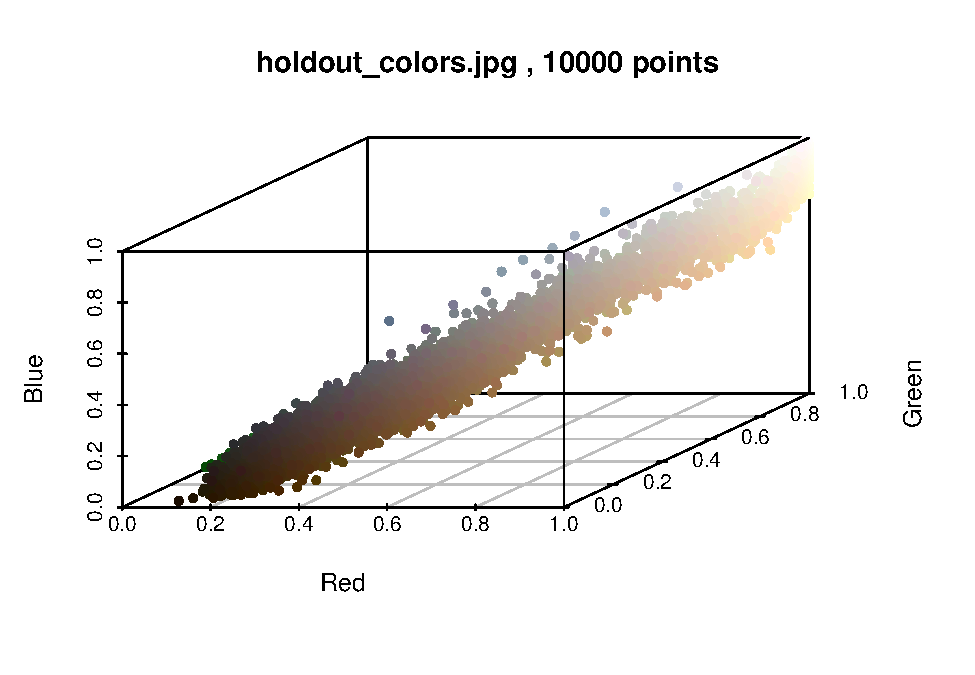
\includegraphics{ProjectPart1_MERGED_files/figure-latex/holdout color plot-1} \end{center}

\begin{Shaded}
\begin{Highlighting}[]
\CommentTok{\# Number of pixels}
\NormalTok{n }\OtherTok{\textless{}{-}} \FunctionTok{nrow}\NormalTok{(train\_data)}
\NormalTok{maxHeight }\OtherTok{\textless{}{-}} \DecValTok{65500}
\NormalTok{height }\OtherTok{\textless{}{-}} \FunctionTok{min}\NormalTok{(n, maxHeight)}
\NormalTok{width }\OtherTok{\textless{}{-}} \FunctionTok{ceiling}\NormalTok{(n }\SpecialCharTok{/}\NormalTok{ height)}
\NormalTok{total\_pixels }\OtherTok{\textless{}{-}}\NormalTok{ height }\SpecialCharTok{*}\NormalTok{ width}

\CommentTok{\# Normalize RGB}
\NormalTok{r }\OtherTok{\textless{}{-}}\NormalTok{ train\_data}\SpecialCharTok{$}\NormalTok{Red }\SpecialCharTok{/} \DecValTok{255}
\NormalTok{g }\OtherTok{\textless{}{-}}\NormalTok{ train\_data}\SpecialCharTok{$}\NormalTok{Green }\SpecialCharTok{/} \DecValTok{255}
\NormalTok{b }\OtherTok{\textless{}{-}}\NormalTok{ train\_data}\SpecialCharTok{$}\NormalTok{Blue }\SpecialCharTok{/} \DecValTok{255}

\CommentTok{\# Calculate padding}
\NormalTok{pad }\OtherTok{\textless{}{-}}\NormalTok{ total\_pixels }\SpecialCharTok{{-}}\NormalTok{ n}

\CommentTok{\# Pad}
\ControlFlowTok{if}\NormalTok{(pad }\SpecialCharTok{\textgreater{}} \DecValTok{0}\NormalTok{)\{}
\NormalTok{  r }\OtherTok{\textless{}{-}} \FunctionTok{c}\NormalTok{(r, }\FunctionTok{rep}\NormalTok{(}\DecValTok{0}\NormalTok{, pad))}
\NormalTok{  g }\OtherTok{\textless{}{-}} \FunctionTok{c}\NormalTok{(g, }\FunctionTok{rep}\NormalTok{(}\DecValTok{1}\NormalTok{, pad))}
\NormalTok{  b }\OtherTok{\textless{}{-}} \FunctionTok{c}\NormalTok{(b, }\FunctionTok{rep}\NormalTok{(}\DecValTok{0}\NormalTok{, pad))}
\NormalTok{\}}

\CommentTok{\# Make array}
\NormalTok{img\_array }\OtherTok{\textless{}{-}} \FunctionTok{array}\NormalTok{(}\FunctionTok{c}\NormalTok{(}\FunctionTok{matrix}\NormalTok{(r, }\AttributeTok{nrow =}\NormalTok{ height, }\AttributeTok{ncol =}\NormalTok{ width),}
                     \FunctionTok{matrix}\NormalTok{(g, }\AttributeTok{nrow =}\NormalTok{ height, }\AttributeTok{ncol =}\NormalTok{ width),}
                     \FunctionTok{matrix}\NormalTok{(b, }\AttributeTok{nrow =}\NormalTok{ height, }\AttributeTok{ncol =}\NormalTok{ width)),}
                   \AttributeTok{dim =} \FunctionTok{c}\NormalTok{(height, width, }\DecValTok{3}\NormalTok{))}

\CommentTok{\# Write to jpg}
\FunctionTok{writeJPEG}\NormalTok{(img\_array, }\AttributeTok{target =} \StringTok{"train\_colors.jpg"}\NormalTok{)}
\end{Highlighting}
\end{Shaded}

\begin{Shaded}
\begin{Highlighting}[]
\NormalTok{image\_path }\OtherTok{\textless{}{-}} \StringTok{"train\_colors.jpg"}
\NormalTok{colordistance}\SpecialCharTok{::}\FunctionTok{plotPixels}\NormalTok{(image\_path)}
\end{Highlighting}
\end{Shaded}

\begin{center}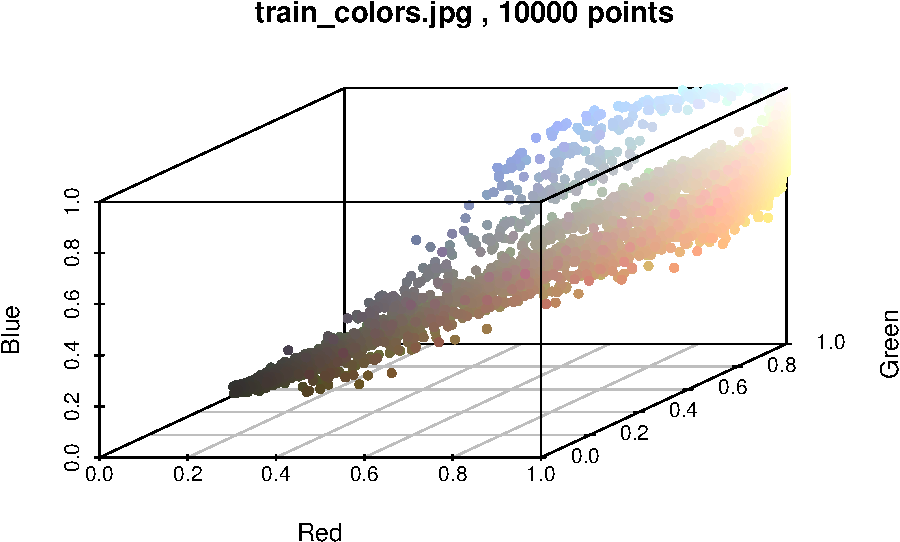
\includegraphics{ProjectPart1_MERGED_files/figure-latex/unnamed-chunk-2-1} \end{center}

\begin{Shaded}
\begin{Highlighting}[]
\NormalTok{bt\_data }\OtherTok{\textless{}{-}}\NormalTok{ holdout\_data }\SpecialCharTok{\%\textgreater{}\%} 
  \FunctionTok{filter}\NormalTok{(BT }\SpecialCharTok{==} \StringTok{"TRUE"}\NormalTok{)}

\NormalTok{n }\OtherTok{\textless{}{-}} \FunctionTok{nrow}\NormalTok{(bt\_data)}
\NormalTok{maxHeight }\OtherTok{\textless{}{-}} \DecValTok{65500}
\NormalTok{height }\OtherTok{\textless{}{-}} \FunctionTok{min}\NormalTok{(n, maxHeight)}
\NormalTok{width }\OtherTok{\textless{}{-}} \FunctionTok{ceiling}\NormalTok{(n }\SpecialCharTok{/}\NormalTok{ height)}
\NormalTok{total\_pixels }\OtherTok{\textless{}{-}}\NormalTok{ height }\SpecialCharTok{*}\NormalTok{ width}

\NormalTok{r }\OtherTok{\textless{}{-}}\NormalTok{ bt\_data}\SpecialCharTok{$}\NormalTok{Red }\SpecialCharTok{/} \DecValTok{255}
\NormalTok{g }\OtherTok{\textless{}{-}}\NormalTok{ bt\_data}\SpecialCharTok{$}\NormalTok{Green }\SpecialCharTok{/} \DecValTok{255}
\NormalTok{b }\OtherTok{\textless{}{-}}\NormalTok{ bt\_data}\SpecialCharTok{$}\NormalTok{Blue }\SpecialCharTok{/} \DecValTok{255}

\NormalTok{pad }\OtherTok{\textless{}{-}}\NormalTok{ total\_pixels }\SpecialCharTok{{-}}\NormalTok{ n}

\ControlFlowTok{if}\NormalTok{(pad }\SpecialCharTok{\textgreater{}} \DecValTok{0}\NormalTok{)\{}
\NormalTok{  r }\OtherTok{\textless{}{-}} \FunctionTok{c}\NormalTok{(r, }\FunctionTok{rep}\NormalTok{(}\DecValTok{0}\NormalTok{, pad))}
\NormalTok{  g }\OtherTok{\textless{}{-}} \FunctionTok{c}\NormalTok{(g, }\FunctionTok{rep}\NormalTok{(}\DecValTok{1}\NormalTok{, pad))}
\NormalTok{  b }\OtherTok{\textless{}{-}} \FunctionTok{c}\NormalTok{(b, }\FunctionTok{rep}\NormalTok{(}\DecValTok{0}\NormalTok{, pad))}
\NormalTok{\}}

\NormalTok{img\_array }\OtherTok{\textless{}{-}} \FunctionTok{array}\NormalTok{(}
  \FunctionTok{c}\NormalTok{(}\FunctionTok{matrix}\NormalTok{(r, }\AttributeTok{nrow =}\NormalTok{ height, }\AttributeTok{ncol =}\NormalTok{ width),}
    \FunctionTok{matrix}\NormalTok{(g, }\AttributeTok{nrow =}\NormalTok{ height, }\AttributeTok{ncol =}\NormalTok{ width),}
    \FunctionTok{matrix}\NormalTok{(b, }\AttributeTok{nrow =}\NormalTok{ height, }\AttributeTok{ncol =}\NormalTok{ width)),}
  \AttributeTok{dim =} \FunctionTok{c}\NormalTok{(height, width, }\DecValTok{3}\NormalTok{)}
\NormalTok{)}

\FunctionTok{writeJPEG}\NormalTok{(img\_array, }\AttributeTok{target =} \StringTok{"holdout\_BT.jpg"}\NormalTok{)}
\end{Highlighting}
\end{Shaded}

\begin{Shaded}
\begin{Highlighting}[]
\NormalTok{image\_path }\OtherTok{\textless{}{-}} \StringTok{"holdout\_BT.jpg"}
\NormalTok{H8hist }\OtherTok{\textless{}{-}}\NormalTok{ colordistance}\SpecialCharTok{::}\FunctionTok{getImageHist}\NormalTok{(image\_path, }\AttributeTok{bins=}\FunctionTok{c}\NormalTok{(}\DecValTok{1}\NormalTok{, }\DecValTok{1}\NormalTok{, }\DecValTok{2}\NormalTok{))}
\end{Highlighting}
\end{Shaded}

\begin{verbatim}
## RGB and HSV are device-dependent, perceptually non-uniform color spaces. See 'Color spaces' vignette for more information.
\end{verbatim}

\begin{verbatim}
## 
## Using 1*1*2 = 2 bins
\end{verbatim}

\begin{center}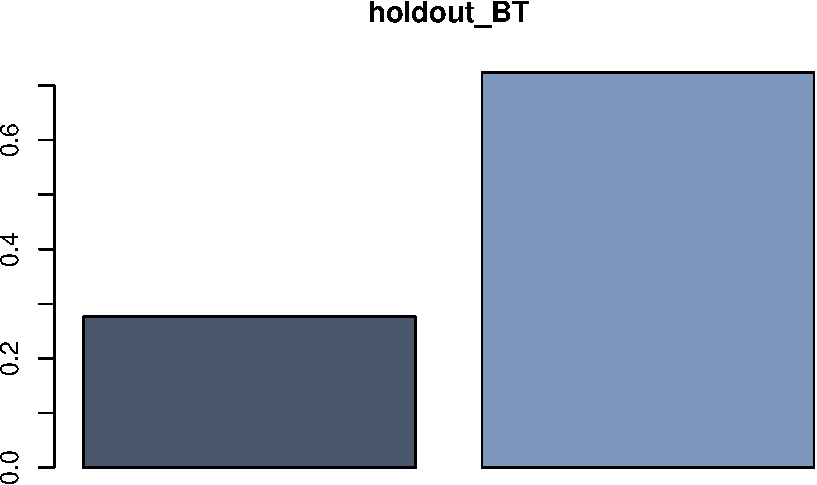
\includegraphics{ProjectPart1_MERGED_files/figure-latex/unnamed-chunk-4-1} \end{center}

\begin{Shaded}
\begin{Highlighting}[]
\NormalTok{bt\_data }\OtherTok{\textless{}{-}}\NormalTok{ train\_data }\SpecialCharTok{\%\textgreater{}\%} 
  \FunctionTok{filter}\NormalTok{(BT }\SpecialCharTok{==} \StringTok{"TRUE"}\NormalTok{)}

\NormalTok{n }\OtherTok{\textless{}{-}} \FunctionTok{nrow}\NormalTok{(bt\_data)}
\NormalTok{maxHeight }\OtherTok{\textless{}{-}} \DecValTok{65500}
\NormalTok{height }\OtherTok{\textless{}{-}} \FunctionTok{min}\NormalTok{(n, maxHeight)}
\NormalTok{width }\OtherTok{\textless{}{-}} \FunctionTok{ceiling}\NormalTok{(n }\SpecialCharTok{/}\NormalTok{ height)}
\NormalTok{total\_pixels }\OtherTok{\textless{}{-}}\NormalTok{ height }\SpecialCharTok{*}\NormalTok{ width}

\NormalTok{r }\OtherTok{\textless{}{-}}\NormalTok{ bt\_data}\SpecialCharTok{$}\NormalTok{Red }\SpecialCharTok{/} \DecValTok{255}
\NormalTok{g }\OtherTok{\textless{}{-}}\NormalTok{ bt\_data}\SpecialCharTok{$}\NormalTok{Green }\SpecialCharTok{/} \DecValTok{255}
\NormalTok{b }\OtherTok{\textless{}{-}}\NormalTok{ bt\_data}\SpecialCharTok{$}\NormalTok{Blue }\SpecialCharTok{/} \DecValTok{255}

\NormalTok{pad }\OtherTok{\textless{}{-}}\NormalTok{ total\_pixels }\SpecialCharTok{{-}}\NormalTok{ n}

\ControlFlowTok{if}\NormalTok{(pad }\SpecialCharTok{\textgreater{}} \DecValTok{0}\NormalTok{)\{}
\NormalTok{  r }\OtherTok{\textless{}{-}} \FunctionTok{c}\NormalTok{(r, }\FunctionTok{rep}\NormalTok{(}\DecValTok{0}\NormalTok{, pad))}
\NormalTok{  g }\OtherTok{\textless{}{-}} \FunctionTok{c}\NormalTok{(g, }\FunctionTok{rep}\NormalTok{(}\DecValTok{1}\NormalTok{, pad))}
\NormalTok{  b }\OtherTok{\textless{}{-}} \FunctionTok{c}\NormalTok{(b, }\FunctionTok{rep}\NormalTok{(}\DecValTok{0}\NormalTok{, pad))}
\NormalTok{\}}

\NormalTok{img\_array }\OtherTok{\textless{}{-}} \FunctionTok{array}\NormalTok{(}
  \FunctionTok{c}\NormalTok{(}\FunctionTok{matrix}\NormalTok{(r, }\AttributeTok{nrow =}\NormalTok{ height, }\AttributeTok{ncol =}\NormalTok{ width),}
    \FunctionTok{matrix}\NormalTok{(g, }\AttributeTok{nrow =}\NormalTok{ height, }\AttributeTok{ncol =}\NormalTok{ width),}
    \FunctionTok{matrix}\NormalTok{(b, }\AttributeTok{nrow =}\NormalTok{ height, }\AttributeTok{ncol =}\NormalTok{ width)),}
  \AttributeTok{dim =} \FunctionTok{c}\NormalTok{(height, width, }\DecValTok{3}\NormalTok{)}
\NormalTok{)}

\FunctionTok{writeJPEG}\NormalTok{(img\_array, }\AttributeTok{target =} \StringTok{"train\_BT.jpg"}\NormalTok{)}
\end{Highlighting}
\end{Shaded}

\begin{Shaded}
\begin{Highlighting}[]
\NormalTok{image\_path }\OtherTok{\textless{}{-}} \StringTok{"train\_BT.jpg"}
\NormalTok{H8hist }\OtherTok{\textless{}{-}}\NormalTok{ colordistance}\SpecialCharTok{::}\FunctionTok{getImageHist}\NormalTok{(image\_path, }\AttributeTok{bins=}\FunctionTok{c}\NormalTok{(}\DecValTok{1}\NormalTok{, }\DecValTok{1}\NormalTok{, }\DecValTok{2}\NormalTok{))}
\end{Highlighting}
\end{Shaded}

\begin{verbatim}
## RGB and HSV are device-dependent, perceptually non-uniform color spaces. See 'Color spaces' vignette for more information.
\end{verbatim}

\begin{verbatim}
## 
## Using 1*1*2 = 2 bins
\end{verbatim}

\begin{center}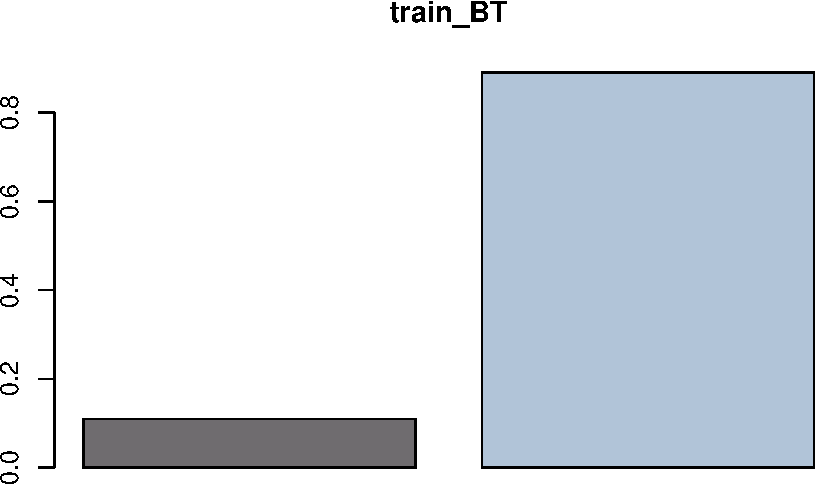
\includegraphics{ProjectPart1_MERGED_files/figure-latex/unnamed-chunk-6-1} \end{center}

Have a look at the distributioin of the two classes for the outcome
named ``BT'' (for BlueTarp).

\begin{Shaded}
\begin{Highlighting}[]
\NormalTok{train\_data }\SpecialCharTok{|\textgreater{}} 
    \FunctionTok{ggplot}\NormalTok{(}\FunctionTok{aes}\NormalTok{(}\AttributeTok{x=}\NormalTok{BT, }\AttributeTok{fill=}\NormalTok{BT)) }\SpecialCharTok{+}
    \FunctionTok{geom\_bar}\NormalTok{(}\AttributeTok{position=}\StringTok{"dodge"}\NormalTok{)}
\end{Highlighting}
\end{Shaded}

\begin{figure}[H]

{\centering 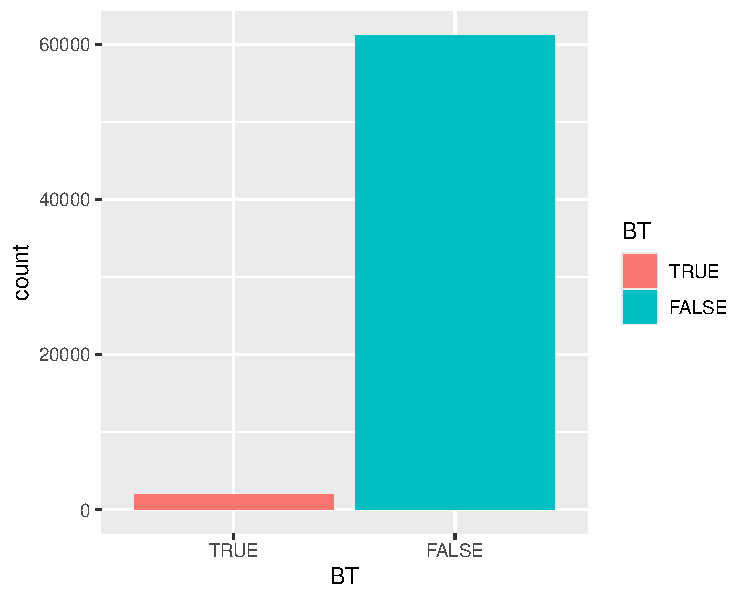
\includegraphics[width=0.6\linewidth]{ProjectPart1_MERGED_files/figure-latex/unnamed-chunk-7-1} 

}

\caption{Distribution of Blue Tarp among all the observations.}\label{fig:unnamed-chunk-7}
\end{figure}

I can see that the two outcome classes are extremely unbalanced. I will
keep this in mind and deal with it later.

\hypertarget{methods}{%
\subsection{Methods}\label{methods}}

\hypertarget{build-three-classification-models-i.e.-lda-qda-and-logistic-regression-with-cross-validation.}{%
\subsubsection{\texorpdfstring{Build three classification models,
\emph{i.e.}, LDA, QDA, and logistic regression, with
cross-validation.}{Build three classification models, i.e., LDA, QDA, and logistic regression, with cross-validation.}}\label{build-three-classification-models-i.e.-lda-qda-and-logistic-regression-with-cross-validation.}}

\hypertarget{prepare-model-workflows}{%
\paragraph{Prepare model workflows}\label{prepare-model-workflows}}

Define the preprocessing steps. In this case, we normalize all numeric
predictors.

\begin{Shaded}
\begin{Highlighting}[]
\CommentTok{\# Formula and recipe}
\NormalTok{formula }\OtherTok{\textless{}{-}}\NormalTok{ BT }\SpecialCharTok{\textasciitilde{}}\NormalTok{ Red }\SpecialCharTok{+}\NormalTok{ Green }\SpecialCharTok{+}\NormalTok{ Blue}
\NormalTok{BT\_recipe }\OtherTok{\textless{}{-}} \FunctionTok{recipe}\NormalTok{(formula, }\AttributeTok{data =}\NormalTok{ train\_data) }\SpecialCharTok{\%\textgreater{}\%}
  \FunctionTok{step\_normalize}\NormalTok{(}\FunctionTok{all\_numeric\_predictors}\NormalTok{())}
\end{Highlighting}
\end{Shaded}

Specify the three models.

\begin{Shaded}
\begin{Highlighting}[]
\CommentTok{\# Specify models}
\NormalTok{logreg\_spec }\OtherTok{\textless{}{-}} \FunctionTok{logistic\_reg}\NormalTok{(}\AttributeTok{mode=}\StringTok{"classification"}\NormalTok{, }\AttributeTok{engine=}\StringTok{"glm"}\NormalTok{)}
\NormalTok{lda\_spec }\OtherTok{\textless{}{-}} \FunctionTok{discrim\_linear}\NormalTok{(}\AttributeTok{mode=}\StringTok{"classification"}\NormalTok{, }\AttributeTok{engine=}\StringTok{"MASS"}\NormalTok{)}
\NormalTok{qda\_spec }\OtherTok{\textless{}{-}} \FunctionTok{discrim\_quad}\NormalTok{(}\AttributeTok{mode=}\StringTok{"classification"}\NormalTok{, }\AttributeTok{engine=}\StringTok{"MASS"}\NormalTok{)}
\end{Highlighting}
\end{Shaded}

Combine preprocessing steps and model specification in workflow.

\begin{Shaded}
\begin{Highlighting}[]
\CommentTok{\# Define workflows}
\NormalTok{logreg\_wf }\OtherTok{\textless{}{-}} \FunctionTok{workflow}\NormalTok{() }\SpecialCharTok{\%\textgreater{}\%}
    \FunctionTok{add\_recipe}\NormalTok{(BT\_recipe) }\SpecialCharTok{\%\textgreater{}\%}
    \FunctionTok{add\_model}\NormalTok{(logreg\_spec)}

\NormalTok{lda\_wf }\OtherTok{\textless{}{-}} \FunctionTok{workflow}\NormalTok{() }\SpecialCharTok{\%\textgreater{}\%}
    \FunctionTok{add\_recipe}\NormalTok{(BT\_recipe) }\SpecialCharTok{\%\textgreater{}\%}
    \FunctionTok{add\_model}\NormalTok{(lda\_spec)}

\NormalTok{qda\_wf }\OtherTok{\textless{}{-}} \FunctionTok{workflow}\NormalTok{() }\SpecialCharTok{\%\textgreater{}\%}
    \FunctionTok{add\_recipe}\NormalTok{(BT\_recipe) }\SpecialCharTok{\%\textgreater{}\%}
    \FunctionTok{add\_model}\NormalTok{(qda\_spec)}
\end{Highlighting}
\end{Shaded}

\hypertarget{cross-validation}{%
\paragraph{Cross-validation}\label{cross-validation}}

Define cross-validation approach - 10-fold cross-validation using
stratified sampling - Measure performance using ROC-AUC (we also collect
accuracy) - Save resample predictions, so that we can build ROC curves
using cross-validation results

\begin{Shaded}
\begin{Highlighting}[]
\CommentTok{\# Define cross{-}validation approach}
\FunctionTok{set.seed}\NormalTok{(}\DecValTok{6030}\NormalTok{)}

\NormalTok{resamples }\OtherTok{\textless{}{-}} \FunctionTok{vfold\_cv}\NormalTok{(train\_data, }\AttributeTok{v =} \DecValTok{10}\NormalTok{, }\AttributeTok{strata =}\NormalTok{ BT)}
\NormalTok{custom\_metrics }\OtherTok{\textless{}{-}} \FunctionTok{metric\_set}\NormalTok{(roc\_auc, accuracy, precision, f\_meas)}
\NormalTok{cv\_control }\OtherTok{\textless{}{-}} \FunctionTok{control\_resamples}\NormalTok{(}\AttributeTok{save\_pred =} \ConstantTok{TRUE}\NormalTok{)}
\end{Highlighting}
\end{Shaded}

Cross-validation

\begin{Shaded}
\begin{Highlighting}[]
\CommentTok{\# Cross{-}validate}
\NormalTok{logreg\_cv }\OtherTok{\textless{}{-}} \FunctionTok{fit\_resamples}\NormalTok{(logreg\_wf, resamples, }\AttributeTok{metrics=}\NormalTok{custom\_metrics, }\AttributeTok{control=}\NormalTok{cv\_control)}
\NormalTok{lda\_cv }\OtherTok{\textless{}{-}} \FunctionTok{fit\_resamples}\NormalTok{(lda\_wf, resamples, }\AttributeTok{metrics=}\NormalTok{custom\_metrics, }\AttributeTok{control=}\NormalTok{cv\_control)}
\NormalTok{qda\_cv }\OtherTok{\textless{}{-}} \FunctionTok{fit\_resamples}\NormalTok{(qda\_wf, resamples, }\AttributeTok{metrics=}\NormalTok{custom\_metrics, }\AttributeTok{control=}\NormalTok{cv\_control)}
\end{Highlighting}
\end{Shaded}

\begin{Shaded}
\begin{Highlighting}[]
\CommentTok{\# Fit to train\_data}
\NormalTok{final\_logreg\_fit }\OtherTok{\textless{}{-}}\NormalTok{ logreg\_wf }\SpecialCharTok{\%\textgreater{}\%} \FunctionTok{fit}\NormalTok{(}\AttributeTok{data =}\NormalTok{ train\_data)}
\end{Highlighting}
\end{Shaded}

\begin{verbatim}
## Warning: glm.fit: fitted probabilities numerically 0 or 1 occurred
\end{verbatim}

\begin{Shaded}
\begin{Highlighting}[]
\NormalTok{final\_lda\_fit    }\OtherTok{\textless{}{-}}\NormalTok{ lda\_wf }\SpecialCharTok{\%\textgreater{}\%} \FunctionTok{fit}\NormalTok{(}\AttributeTok{data =}\NormalTok{ train\_data)}
\NormalTok{final\_qda\_fit    }\OtherTok{\textless{}{-}}\NormalTok{ qda\_wf }\SpecialCharTok{\%\textgreater{}\%} \FunctionTok{fit}\NormalTok{(}\AttributeTok{data =}\NormalTok{ train\_data)}
\end{Highlighting}
\end{Shaded}

\hypertarget{model-performance-before-threshold-selection}{%
\subsubsection{Model performance before threshold
selection}\label{model-performance-before-threshold-selection}}

The performance metrics estimated using 10-fold cross-validation.

\begin{Shaded}
\begin{Highlighting}[]
\NormalTok{cv\_metrics }\OtherTok{\textless{}{-}} \FunctionTok{bind\_rows}\NormalTok{(}
    \FunctionTok{collect\_metrics}\NormalTok{(logreg\_cv) }\SpecialCharTok{\%\textgreater{}\%}
        \FunctionTok{mutate}\NormalTok{(}\AttributeTok{model=}\StringTok{"Logistic regression"}\NormalTok{),}
    \FunctionTok{collect\_metrics}\NormalTok{(lda\_cv) }\SpecialCharTok{\%\textgreater{}\%}
        \FunctionTok{mutate}\NormalTok{(}\AttributeTok{model=}\StringTok{"LDA"}\NormalTok{),}
    \FunctionTok{collect\_metrics}\NormalTok{(qda\_cv) }\SpecialCharTok{\%\textgreater{}\%}
        \FunctionTok{mutate}\NormalTok{(}\AttributeTok{model=}\StringTok{"QDA"}\NormalTok{)}
\NormalTok{)}

\NormalTok{cv\_metrics }\SpecialCharTok{\%\textgreater{}\%}
    \FunctionTok{select}\NormalTok{(model, .metric, mean) }\SpecialCharTok{\%\textgreater{}\%}
    \FunctionTok{pivot\_wider}\NormalTok{(}\AttributeTok{names\_from=}\StringTok{".metric"}\NormalTok{, }\AttributeTok{values\_from=}\StringTok{"mean"}\NormalTok{) }\SpecialCharTok{\%\textgreater{}\%}
\NormalTok{    knitr}\SpecialCharTok{::}\FunctionTok{kable}\NormalTok{(}
      \AttributeTok{caption=}\StringTok{"Cross{-}validation performance metrics."}\NormalTok{, }
      \AttributeTok{digits=}\DecValTok{3}\NormalTok{,}
      \AttributeTok{col.names =} \FunctionTok{c}\NormalTok{(}\StringTok{"Model"}\NormalTok{, }\StringTok{"Accuracy"}\NormalTok{, }\StringTok{"F{-}measure"}\NormalTok{, }\StringTok{"Precision"}\NormalTok{, }\StringTok{"ROC{-}AUC"}\NormalTok{)}
\NormalTok{  ) }\SpecialCharTok{\%\textgreater{}\%}
\NormalTok{  kableExtra}\SpecialCharTok{::}\FunctionTok{kable\_styling}\NormalTok{(}\AttributeTok{full\_width =} \ConstantTok{FALSE}\NormalTok{, }\AttributeTok{position =} \StringTok{"center"}\NormalTok{)}
\end{Highlighting}
\end{Shaded}

\begin{longtable}[t]{lrrrr}
\caption{\label{tab:cv metrics}Cross-validation performance metrics.}\\
\toprule
Model & Accuracy & F-measure & Precision & ROC-AUC\\
\midrule
Logistic regression & 0.995 & 0.923 & 0.964 & 0.998\\
LDA & 0.984 & 0.761 & 0.725 & 0.989\\
QDA & 0.995 & 0.908 & 0.989 & 0.998\\
\bottomrule
\end{longtable}

Visualization of the same data

\begin{Shaded}
\begin{Highlighting}[]
\FunctionTok{ggplot}\NormalTok{(cv\_metrics, }\FunctionTok{aes}\NormalTok{(}\AttributeTok{x=}\NormalTok{mean, }\AttributeTok{y=}\NormalTok{model, }\AttributeTok{xmin=}\NormalTok{mean }\SpecialCharTok{{-}}\NormalTok{ std\_err, }\AttributeTok{xmax=}\NormalTok{mean }\SpecialCharTok{+}\NormalTok{ std\_err)) }\SpecialCharTok{+}
    \FunctionTok{geom\_point}\NormalTok{() }\SpecialCharTok{+}
    \FunctionTok{geom\_linerange}\NormalTok{() }\SpecialCharTok{+}
    \FunctionTok{facet\_wrap}\NormalTok{(}\SpecialCharTok{\textasciitilde{}}\NormalTok{ .metric)}
\end{Highlighting}
\end{Shaded}

\begin{figure}[H]

{\centering 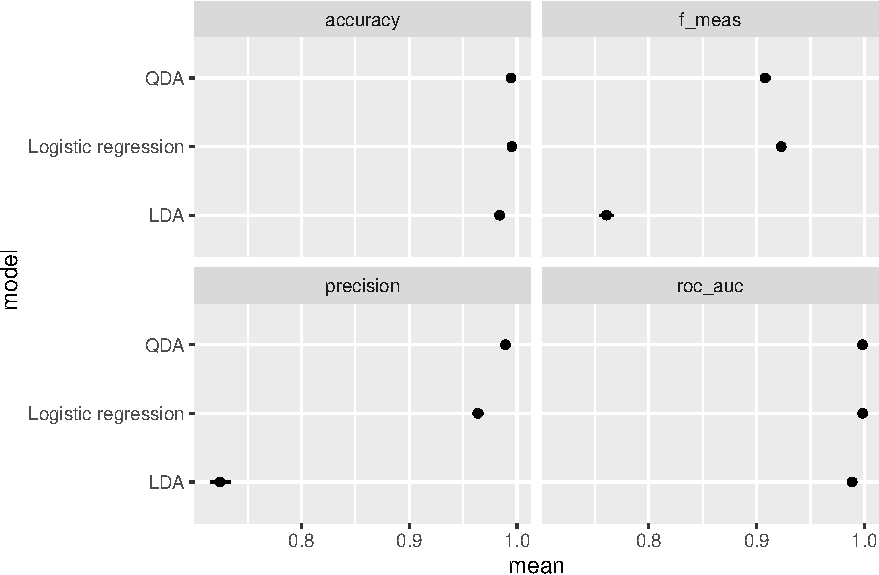
\includegraphics[width=0.75\linewidth]{ProjectPart1_MERGED_files/figure-latex/cv-metrics-figure-1} 

}

\caption{Cross-validation performance metrics}\label{fig:cv-metrics-figure}
\end{figure}

Cross-validation ROC curves

\begin{Shaded}
\begin{Highlighting}[]
\FunctionTok{bind\_rows}\NormalTok{(}
    \FunctionTok{collect\_predictions}\NormalTok{(logreg\_cv) }\SpecialCharTok{\%\textgreater{}\%} \FunctionTok{mutate}\NormalTok{(}\AttributeTok{model=}\StringTok{"Logistic regression"}\NormalTok{),}
    \FunctionTok{collect\_predictions}\NormalTok{(lda\_cv) }\SpecialCharTok{\%\textgreater{}\%} \FunctionTok{mutate}\NormalTok{(}\AttributeTok{model=}\StringTok{"LDA"}\NormalTok{),}
    \FunctionTok{collect\_predictions}\NormalTok{(qda\_cv) }\SpecialCharTok{\%\textgreater{}\%} \FunctionTok{mutate}\NormalTok{(}\AttributeTok{model=}\StringTok{"QDA"}\NormalTok{)}
\NormalTok{) }\SpecialCharTok{\%\textgreater{}\%}
    \FunctionTok{group\_by}\NormalTok{(model) }\SpecialCharTok{\%\textgreater{}\%}
    \FunctionTok{roc\_curve}\NormalTok{(}\AttributeTok{truth=}\NormalTok{BT, .pred\_TRUE, }\AttributeTok{event\_level=}\StringTok{"first"}\NormalTok{) }\SpecialCharTok{\%\textgreater{}\%}
    \FunctionTok{autoplot}\NormalTok{()}
\end{Highlighting}
\end{Shaded}

\begin{figure}[H]

{\centering 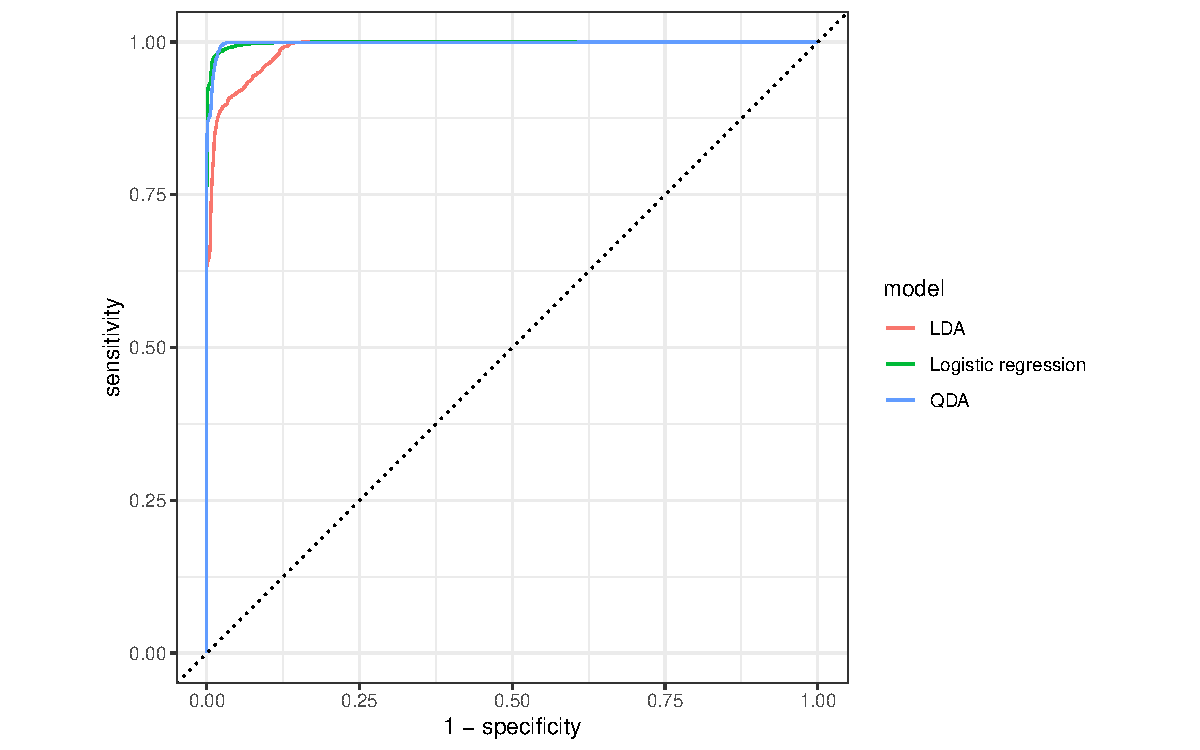
\includegraphics{ProjectPart1_MERGED_files/figure-latex/cv-roc-curves-overlay-1} 

}

\caption{Overlay of cross-validation ROC curves}\label{fig:cv-roc-curves-overlay}
\end{figure}

\hypertarget{threshold-selectionoptimization}{%
\subsubsection{Threshold
selection/Optimization}\label{threshold-selectionoptimization}}

It is clear that our outcome classes are heavily imbalanced, so we need
to adjust the threshold to improve its predictive accuracy and
precision.

Use package \texttt{probably} to explore the threshold. We define two
functions to look at the effect of threshold selection on performance
metrics and the associated confusion matrices:

\begin{Shaded}
\begin{Highlighting}[]
\CommentTok{\# Create metric set}
\NormalTok{class\_metrics }\OtherTok{\textless{}{-}} \FunctionTok{metric\_set}\NormalTok{(accuracy, sens, f\_meas)}

\CommentTok{\# Compute metrics}
\NormalTok{compute\_my\_metrics }\OtherTok{\textless{}{-}} \ControlFlowTok{function}\NormalTok{(data) \{}
\NormalTok{  res\_class }\OtherTok{\textless{}{-}} \FunctionTok{class\_metrics}\NormalTok{(data, }\AttributeTok{truth =}\NormalTok{ BT, }\AttributeTok{estimate =}\NormalTok{ .pred\_class)}
\NormalTok{  res\_prob  }\OtherTok{\textless{}{-}} \FunctionTok{roc\_auc}\NormalTok{(data, }\AttributeTok{truth =}\NormalTok{ BT, .pred\_TRUE, }\AttributeTok{event\_level =} \StringTok{"first"}\NormalTok{)}
  \FunctionTok{bind\_rows}\NormalTok{(res\_class, res\_prob)}
\NormalTok{\}}
\end{Highlighting}
\end{Shaded}

\begin{Shaded}
\begin{Highlighting}[]
\NormalTok{calculate\_metrics\_cv }\OtherTok{\textless{}{-}} \ControlFlowTok{function}\NormalTok{(cv\_object, holdout, model\_name, workflow, train\_data) \{}
  \CommentTok{\# Use CV preds}
\NormalTok{  train\_aug }\OtherTok{\textless{}{-}} \FunctionTok{collect\_predictions}\NormalTok{(cv\_object)}
  
  \CommentTok{\# Augment with holdout}
\NormalTok{  final\_fit   }\OtherTok{\textless{}{-}}\NormalTok{ workflow }\SpecialCharTok{\%\textgreater{}\%} \FunctionTok{fit}\NormalTok{(train\_data)}
\NormalTok{  holdout\_aug }\OtherTok{\textless{}{-}} \FunctionTok{augment}\NormalTok{(final\_fit, }\AttributeTok{new\_data =}\NormalTok{ holdout)}
  
  \FunctionTok{bind\_rows}\NormalTok{(}
    \FunctionTok{bind\_cols}\NormalTok{(}
      \AttributeTok{model   =}\NormalTok{ model\_name,}
      \AttributeTok{dataset =} \StringTok{"train"}\NormalTok{,}
      \FunctionTok{compute\_my\_metrics}\NormalTok{(train\_aug)}
\NormalTok{    ),}
    \FunctionTok{bind\_cols}\NormalTok{(}
      \AttributeTok{model   =}\NormalTok{ model\_name,}
      \AttributeTok{dataset =} \StringTok{"holdout"}\NormalTok{,}
      \FunctionTok{compute\_my\_metrics}\NormalTok{(holdout\_aug)}
\NormalTok{    )}
\NormalTok{  )}
\NormalTok{\}}
\end{Highlighting}
\end{Shaded}

\begin{Shaded}
\begin{Highlighting}[]
\NormalTok{all\_metrics }\OtherTok{\textless{}{-}} \FunctionTok{bind\_rows}\NormalTok{(}
    \FunctionTok{calculate\_metrics\_cv}\NormalTok{(logreg\_cv, holdout\_data, }\StringTok{"logreg"}\NormalTok{, logreg\_wf, train\_data),}
    \FunctionTok{calculate\_metrics\_cv}\NormalTok{(lda\_cv, holdout\_data, }\StringTok{"LDA"}\NormalTok{, lda\_wf, train\_data),}
    \FunctionTok{calculate\_metrics\_cv}\NormalTok{(qda\_cv, holdout\_data, }\StringTok{"QDA"}\NormalTok{, qda\_wf, train\_data)}
\NormalTok{) }\SpecialCharTok{\%\textgreater{}\%} \FunctionTok{arrange}\NormalTok{(dataset)}
\end{Highlighting}
\end{Shaded}

\begin{verbatim}
## Warning: glm.fit: fitted probabilities numerically 0 or 1 occurred
\end{verbatim}

\begin{Shaded}
\begin{Highlighting}[]
\NormalTok{all\_metrics }\SpecialCharTok{\%\textgreater{}\%}
        \FunctionTok{pivot\_wider}\NormalTok{(}\AttributeTok{names\_from=}\NormalTok{.metric, }\AttributeTok{values\_from=}\NormalTok{.estimate) }\SpecialCharTok{\%\textgreater{}\%}
        \FunctionTok{select}\NormalTok{(}\SpecialCharTok{{-}}\NormalTok{.estimator) }\SpecialCharTok{\%\textgreater{}\%}
\NormalTok{        knitr}\SpecialCharTok{::}\FunctionTok{kable}\NormalTok{(}
          \AttributeTok{caption=} \StringTok{"Metrics for the classification models."}\NormalTok{, }
          \AttributeTok{digits=}\DecValTok{3}\NormalTok{) }\SpecialCharTok{\%\textgreater{}\%}
\NormalTok{        kableExtra}\SpecialCharTok{::}\FunctionTok{kable\_styling}\NormalTok{(}\AttributeTok{full\_width=}\ConstantTok{FALSE}\NormalTok{)}
\end{Highlighting}
\end{Shaded}

\begin{longtable}[t]{llrrrr}
\caption{\label{tab:metrics table 2}Metrics for the classification models.}\\
\toprule
model & dataset & accuracy & sens & f\_meas & roc\_auc\\
\midrule
logreg & holdout & 0.990 & 0.988 & 0.583 & 0.999\\
LDA & holdout & 0.982 & 0.839 & 0.399 & 0.992\\
QDA & holdout & 0.996 & 0.695 & 0.714 & 0.992\\
logreg & train & 0.995 & 0.886 & 0.923 & 0.998\\
LDA & train & 0.984 & 0.801 & 0.761 & 0.989\\
\addlinespace
QDA & train & 0.995 & 0.839 & 0.908 & 0.998\\
\bottomrule
\end{longtable}

\begin{Shaded}
\begin{Highlighting}[]
\NormalTok{threshold\_graph }\OtherTok{\textless{}{-}} \ControlFlowTok{function}\NormalTok{(model\_cv, model\_name) \{}
\NormalTok{    performance }\OtherTok{\textless{}{-}}\NormalTok{ probably}\SpecialCharTok{::}\FunctionTok{threshold\_perf}\NormalTok{(}\FunctionTok{collect\_predictions}\NormalTok{(model\_cv), BT, .pred\_TRUE,}
        \AttributeTok{thresholds=}\FunctionTok{seq}\NormalTok{(}\FloatTok{0.01}\NormalTok{, }\FloatTok{0.99}\NormalTok{, }\FloatTok{0.01}\NormalTok{), }\AttributeTok{event\_level=}\StringTok{"first"}\NormalTok{,}
        \AttributeTok{metrics=}\FunctionTok{metric\_set}\NormalTok{(f\_meas, accuracy, sens))}
\NormalTok{    max\_metrics }\OtherTok{\textless{}{-}}\NormalTok{ performance }\SpecialCharTok{\%\textgreater{}\%}
        \FunctionTok{drop\_na}\NormalTok{() }\SpecialCharTok{\%\textgreater{}\%}
        \FunctionTok{group\_by}\NormalTok{(.metric) }\SpecialCharTok{\%\textgreater{}\%}
        \FunctionTok{filter}\NormalTok{(.estimate }\SpecialCharTok{==} \FunctionTok{max}\NormalTok{(.estimate))}
\NormalTok{    g }\OtherTok{\textless{}{-}} \FunctionTok{ggplot}\NormalTok{(performance, }\FunctionTok{aes}\NormalTok{(}\AttributeTok{x=}\NormalTok{.threshold, }\AttributeTok{y=}\NormalTok{.estimate, }\AttributeTok{color=}\NormalTok{.metric)) }\SpecialCharTok{+}
        \FunctionTok{geom\_line}\NormalTok{() }\SpecialCharTok{+}
        \FunctionTok{geom\_point}\NormalTok{(}\AttributeTok{data=}\NormalTok{max\_metrics, }\AttributeTok{color=}\StringTok{"black"}\NormalTok{) }\SpecialCharTok{+}
        \FunctionTok{labs}\NormalTok{(}\AttributeTok{title=}\NormalTok{model\_name, }\AttributeTok{x=}\StringTok{"Threshold"}\NormalTok{, }\AttributeTok{y=}\StringTok{"Metric value"}\NormalTok{) }\SpecialCharTok{+}
        \FunctionTok{coord\_cartesian}\NormalTok{(}\AttributeTok{ylim=}\FunctionTok{c}\NormalTok{(}\DecValTok{0}\NormalTok{, }\DecValTok{1}\NormalTok{))}
\NormalTok{    thresholds }\OtherTok{\textless{}{-}}\NormalTok{ max\_metrics }\SpecialCharTok{\%\textgreater{}\%}
        \FunctionTok{select}\NormalTok{(.metric, .threshold) }\SpecialCharTok{\%\textgreater{}\%}
        \FunctionTok{deframe}\NormalTok{()}
    \FunctionTok{return}\NormalTok{(}\FunctionTok{list}\NormalTok{(}\AttributeTok{graph=}\NormalTok{g, }\AttributeTok{thresholds=}\NormalTok{thresholds))}
\NormalTok{\}}

\NormalTok{visualize\_conf\_mat }\OtherTok{\textless{}{-}} \ControlFlowTok{function}\NormalTok{(model\_cv, thresholds, metric) \{}
\NormalTok{    threshold }\OtherTok{\textless{}{-}}\NormalTok{ thresholds[metric]}
\NormalTok{    cm }\OtherTok{\textless{}{-}} \FunctionTok{collect\_predictions}\NormalTok{(logreg\_cv) }\SpecialCharTok{\%\textgreater{}\%}
        \FunctionTok{mutate}\NormalTok{(}
            \AttributeTok{.pred\_class =} \FunctionTok{make\_two\_class\_pred}\NormalTok{(.pred\_TRUE, }\FunctionTok{c}\NormalTok{(}\StringTok{"TRUE"}\NormalTok{, }\StringTok{"FALSE"}\NormalTok{), }\AttributeTok{threshold=}\NormalTok{threshold),}
\NormalTok{        ) }\SpecialCharTok{\%\textgreater{}\%}
        \FunctionTok{conf\_mat}\NormalTok{(}\AttributeTok{truth=}\NormalTok{BT, }\AttributeTok{estimate=}\NormalTok{.pred\_class)}
    \FunctionTok{autoplot}\NormalTok{(cm, }\AttributeTok{type=}\StringTok{"heatmap"}\NormalTok{) }\SpecialCharTok{+}
        \FunctionTok{labs}\NormalTok{(}\AttributeTok{title=}\FunctionTok{sprintf}\NormalTok{(}\StringTok{"Threshold \%.2f (\%s)"}\NormalTok{, threshold, metric))}
\NormalTok{\}}

\NormalTok{overview\_model }\OtherTok{\textless{}{-}} \ControlFlowTok{function}\NormalTok{(model\_cv, model\_name) \{}
\NormalTok{    tg }\OtherTok{\textless{}{-}} \FunctionTok{threshold\_graph}\NormalTok{(model\_cv, model\_name)}
\NormalTok{    g1 }\OtherTok{\textless{}{-}} \FunctionTok{visualize\_conf\_mat}\NormalTok{(model\_cv, tg}\SpecialCharTok{$}\NormalTok{thresholds, }\StringTok{"accuracy"}\NormalTok{)}
\NormalTok{    g2 }\OtherTok{\textless{}{-}} \FunctionTok{visualize\_conf\_mat}\NormalTok{(model\_cv, tg}\SpecialCharTok{$}\NormalTok{thresholds, }\StringTok{"f\_meas"}\NormalTok{)}
\NormalTok{    g3 }\OtherTok{\textless{}{-}} \FunctionTok{visualize\_conf\_mat}\NormalTok{(model\_cv, tg}\SpecialCharTok{$}\NormalTok{thresholds, }\StringTok{"sens"}\NormalTok{)}
\NormalTok{    tg}\SpecialCharTok{$}\NormalTok{graph }\SpecialCharTok{+}\NormalTok{ (g1 }\SpecialCharTok{/}\NormalTok{ g2 }\SpecialCharTok{/}\NormalTok{ g3)}
\NormalTok{\}}
\end{Highlighting}
\end{Shaded}

Notes:

\begin{itemize}
\tightlist
\item
  \texttt{f\_meas} cannot be calculated for high threshold values. In
  this case, the function \texttt{threshold\_perf} returns \texttt{NA}
  for the F-measure. We filter out these values using
  \texttt{drop\_na()}.
\end{itemize}

\begin{Shaded}
\begin{Highlighting}[]
\NormalTok{g1 }\OtherTok{\textless{}{-}} \FunctionTok{overview\_model}\NormalTok{(logreg\_cv, }\StringTok{"Logistic regression"}\NormalTok{)}
\NormalTok{g2 }\OtherTok{\textless{}{-}} \FunctionTok{overview\_model}\NormalTok{(lda\_cv, }\StringTok{"LDA"}\NormalTok{)}
\NormalTok{g3 }\OtherTok{\textless{}{-}} \FunctionTok{overview\_model}\NormalTok{(qda\_cv, }\StringTok{"QDA"}\NormalTok{)}

\NormalTok{g1 }\SpecialCharTok{/}\NormalTok{ g2 }\SpecialCharTok{/}\NormalTok{ g3}
\end{Highlighting}
\end{Shaded}

\begin{figure}[H]

{\centering 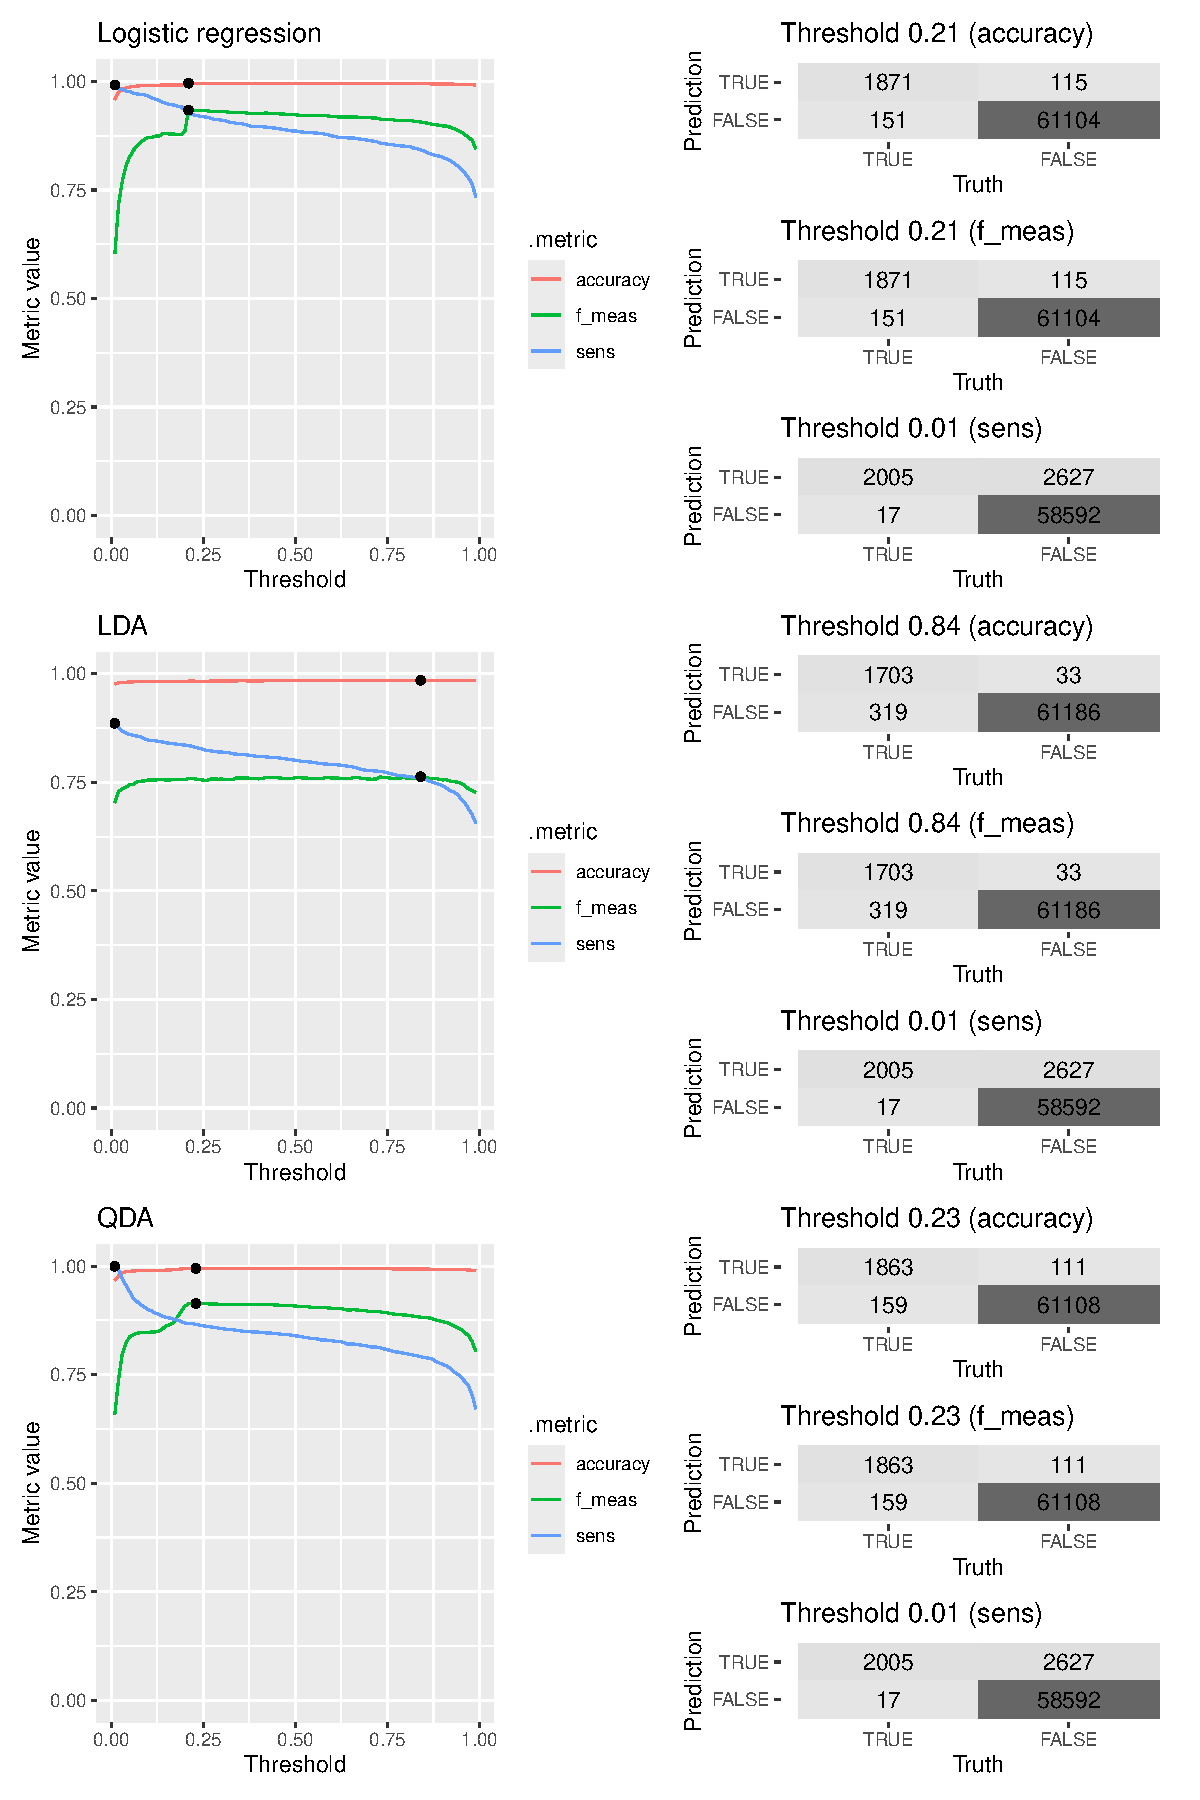
\includegraphics[width=0.8\linewidth]{ProjectPart1_MERGED_files/figure-latex/print threshold graphs-1} 

}

\caption{Metrics as a function of model performance}\label{fig:print threshold graphs}
\end{figure}

\begin{Shaded}
\begin{Highlighting}[]
\CommentTok{\# Tweak f measure}
\NormalTok{f\_meas\_adj2 }\OtherTok{\textless{}{-}} \FunctionTok{metric\_tweak}\NormalTok{(}\StringTok{"f\_meas\_adj2"}\NormalTok{, f\_meas, }\AttributeTok{beta =} \DecValTok{2}\NormalTok{)}
\NormalTok{f\_meas\_adj3 }\OtherTok{\textless{}{-}} \FunctionTok{metric\_tweak}\NormalTok{(}\StringTok{"f\_meas\_adj3"}\NormalTok{, f\_meas, }\AttributeTok{beta =} \DecValTok{3}\NormalTok{)}

\NormalTok{threshold\_graph }\OtherTok{\textless{}{-}} \ControlFlowTok{function}\NormalTok{(model\_cv, model\_name) \{}
\NormalTok{    performance }\OtherTok{\textless{}{-}}\NormalTok{ probably}\SpecialCharTok{::}\FunctionTok{threshold\_perf}\NormalTok{(}\FunctionTok{collect\_predictions}\NormalTok{(model\_cv), BT, .pred\_TRUE,}
        \AttributeTok{thresholds=}\FunctionTok{seq}\NormalTok{(}\FloatTok{0.01}\NormalTok{, }\FloatTok{0.99}\NormalTok{, }\FloatTok{0.01}\NormalTok{), }\AttributeTok{event\_level=}\StringTok{"first"}\NormalTok{,}
        \AttributeTok{metrics=}\FunctionTok{metric\_set}\NormalTok{(f\_meas, f\_meas\_adj2, f\_meas\_adj3))}
\NormalTok{    max\_metrics }\OtherTok{\textless{}{-}}\NormalTok{ performance }\SpecialCharTok{\%\textgreater{}\%}
        \FunctionTok{drop\_na}\NormalTok{() }\SpecialCharTok{\%\textgreater{}\%}
        \FunctionTok{group\_by}\NormalTok{(.metric) }\SpecialCharTok{\%\textgreater{}\%}
        \FunctionTok{filter}\NormalTok{(.estimate }\SpecialCharTok{==} \FunctionTok{max}\NormalTok{(.estimate))}
\NormalTok{    g }\OtherTok{\textless{}{-}} \FunctionTok{ggplot}\NormalTok{(performance, }\FunctionTok{aes}\NormalTok{(}\AttributeTok{x=}\NormalTok{.threshold, }\AttributeTok{y=}\NormalTok{.estimate, }\AttributeTok{color=}\NormalTok{.metric)) }\SpecialCharTok{+}
        \FunctionTok{geom\_line}\NormalTok{() }\SpecialCharTok{+}
        \FunctionTok{geom\_point}\NormalTok{(}\AttributeTok{data=}\NormalTok{max\_metrics, }\AttributeTok{color=}\StringTok{"black"}\NormalTok{) }\SpecialCharTok{+}
        \FunctionTok{labs}\NormalTok{(}\AttributeTok{title=}\NormalTok{model\_name, }\AttributeTok{x=}\StringTok{"Threshold"}\NormalTok{, }\AttributeTok{y=}\StringTok{"Metric value"}\NormalTok{) }\SpecialCharTok{+}
        \FunctionTok{coord\_cartesian}\NormalTok{(}\AttributeTok{ylim=}\FunctionTok{c}\NormalTok{(}\DecValTok{0}\NormalTok{, }\DecValTok{1}\NormalTok{))}
\NormalTok{    thresholds }\OtherTok{\textless{}{-}}\NormalTok{ max\_metrics }\SpecialCharTok{\%\textgreater{}\%}
        \FunctionTok{select}\NormalTok{(.metric, .threshold) }\SpecialCharTok{\%\textgreater{}\%}
        \FunctionTok{deframe}\NormalTok{()}
    \FunctionTok{return}\NormalTok{(}\FunctionTok{list}\NormalTok{(}\AttributeTok{graph=}\NormalTok{g, }\AttributeTok{thresholds=}\NormalTok{thresholds))}
\NormalTok{\}}

\NormalTok{visualize\_conf\_mat }\OtherTok{\textless{}{-}} \ControlFlowTok{function}\NormalTok{(model\_cv, thresholds, metric) \{}
\NormalTok{    threshold }\OtherTok{\textless{}{-}}\NormalTok{ thresholds[metric]}
\NormalTok{    cm }\OtherTok{\textless{}{-}} \FunctionTok{collect\_predictions}\NormalTok{(logreg\_cv) }\SpecialCharTok{\%\textgreater{}\%}
        \FunctionTok{mutate}\NormalTok{(}
            \AttributeTok{.pred\_class =} \FunctionTok{make\_two\_class\_pred}\NormalTok{(.pred\_TRUE, }\FunctionTok{c}\NormalTok{(}\StringTok{"TRUE"}\NormalTok{, }\StringTok{"FALSE"}\NormalTok{), }\AttributeTok{threshold=}\NormalTok{threshold),}
\NormalTok{        ) }\SpecialCharTok{\%\textgreater{}\%}
        \FunctionTok{conf\_mat}\NormalTok{(}\AttributeTok{truth=}\NormalTok{BT, }\AttributeTok{estimate=}\NormalTok{.pred\_class)}
    \FunctionTok{autoplot}\NormalTok{(cm, }\AttributeTok{type=}\StringTok{"heatmap"}\NormalTok{) }\SpecialCharTok{+}
        \FunctionTok{labs}\NormalTok{(}\AttributeTok{title=}\FunctionTok{sprintf}\NormalTok{(}\StringTok{"Threshold \%.2f (\%s)"}\NormalTok{, threshold, metric))}
\NormalTok{\}}

\NormalTok{overview\_model }\OtherTok{\textless{}{-}} \ControlFlowTok{function}\NormalTok{(model\_cv, model\_name) \{}
\NormalTok{    tg }\OtherTok{\textless{}{-}} \FunctionTok{threshold\_graph}\NormalTok{(model\_cv, model\_name)}
\NormalTok{    g1 }\OtherTok{\textless{}{-}} \FunctionTok{visualize\_conf\_mat}\NormalTok{(model\_cv, tg}\SpecialCharTok{$}\NormalTok{thresholds, }\StringTok{"f\_meas"}\NormalTok{)}
\NormalTok{    g2 }\OtherTok{\textless{}{-}} \FunctionTok{visualize\_conf\_mat}\NormalTok{(model\_cv, tg}\SpecialCharTok{$}\NormalTok{thresholds, }\StringTok{"f\_meas\_adj2"}\NormalTok{)}
\NormalTok{    g3 }\OtherTok{\textless{}{-}} \FunctionTok{visualize\_conf\_mat}\NormalTok{(model\_cv, tg}\SpecialCharTok{$}\NormalTok{thresholds, }\StringTok{"f\_meas\_adj3"}\NormalTok{)}
\NormalTok{    tg}\SpecialCharTok{$}\NormalTok{graph }\SpecialCharTok{+}\NormalTok{ (g1 }\SpecialCharTok{/}\NormalTok{ g2 }\SpecialCharTok{/}\NormalTok{ g3)}
\NormalTok{\}}
\end{Highlighting}
\end{Shaded}

\begin{Shaded}
\begin{Highlighting}[]
\NormalTok{g1 }\OtherTok{\textless{}{-}} \FunctionTok{overview\_model}\NormalTok{(logreg\_cv, }\StringTok{"Logistic regression"}\NormalTok{)}
\NormalTok{g2 }\OtherTok{\textless{}{-}} \FunctionTok{overview\_model}\NormalTok{(lda\_cv, }\StringTok{"LDA"}\NormalTok{)}
\NormalTok{g3 }\OtherTok{\textless{}{-}} \FunctionTok{overview\_model}\NormalTok{(qda\_cv, }\StringTok{"QDA"}\NormalTok{)}

\NormalTok{g1 }\SpecialCharTok{/}\NormalTok{ g2 }\SpecialCharTok{/}\NormalTok{ g3}
\end{Highlighting}
\end{Shaded}

\begin{figure}[H]

{\centering 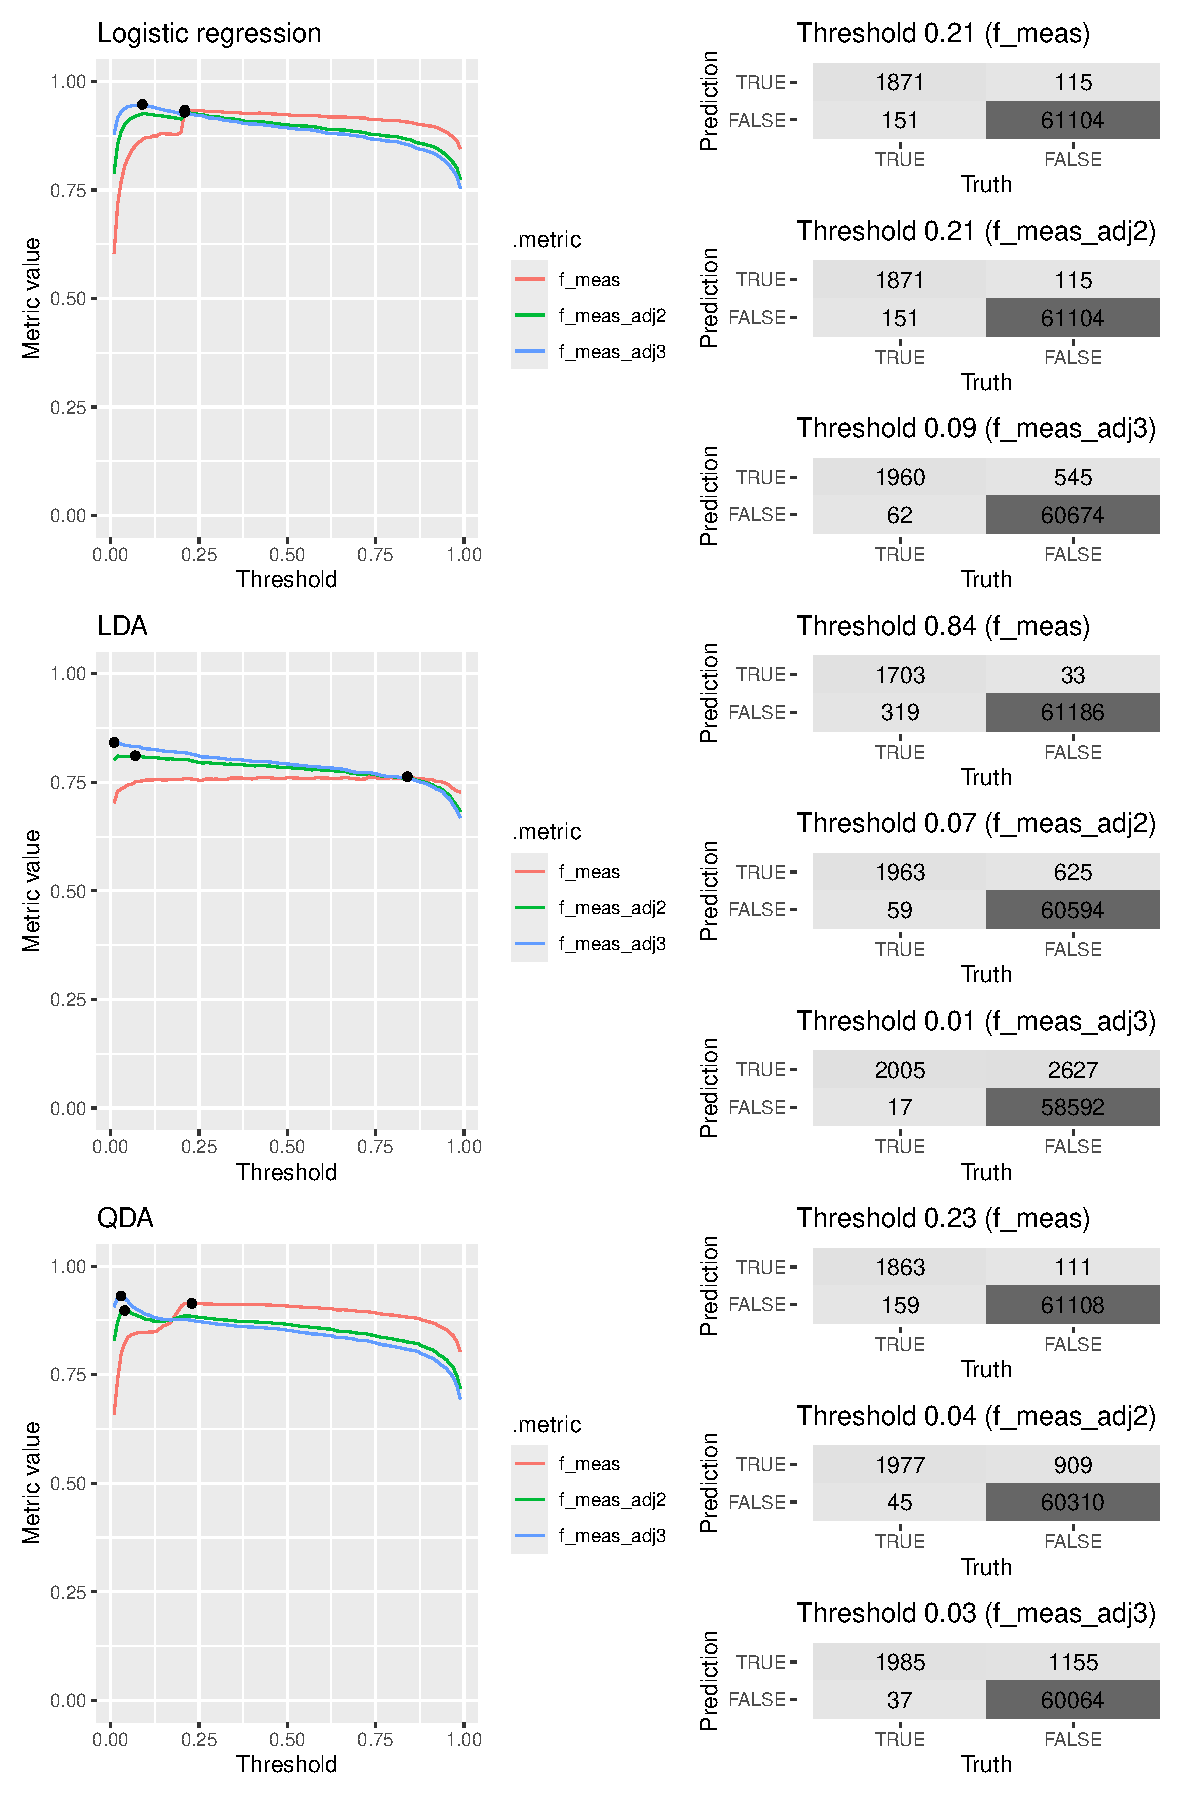
\includegraphics[width=0.8\linewidth]{ProjectPart1_MERGED_files/figure-latex/print threshold graphs f_meas-1} 

}

\caption{Metrics as a function of model performance}\label{fig:print threshold graphs f_meas}
\end{figure}

Next, I compared the ROC curves for the logistic regression between the
cross-validation predictions and the predictions on the full training
data set to see if the logistic regression was overfitting the training
data.

\begin{Shaded}
\begin{Highlighting}[]
\CommentTok{\# Generate ROC plot}
\NormalTok{get\_roc\_overlay\_autoplot }\OtherTok{\textless{}{-}} \ControlFlowTok{function}\NormalTok{(cv\_object, wf, data, model\_name) \{}
  \CommentTok{\# Fit the full model}
\NormalTok{  full\_fit }\OtherTok{\textless{}{-}}\NormalTok{ wf }\SpecialCharTok{\%\textgreater{}\%} \FunctionTok{fit}\NormalTok{(data)}
  
  \CommentTok{\# Get CV preds}
\NormalTok{  cv\_preds }\OtherTok{\textless{}{-}} \FunctionTok{collect\_predictions}\NormalTok{(cv\_object) }\SpecialCharTok{\%\textgreater{}\%} 
    \FunctionTok{mutate}\NormalTok{(}\AttributeTok{source =} \StringTok{"CV"}\NormalTok{)}
  
  \CommentTok{\# Get preds for full model}
\NormalTok{  full\_preds }\OtherTok{\textless{}{-}} \FunctionTok{augment}\NormalTok{(full\_fit, }\AttributeTok{new\_data =}\NormalTok{ data) }\SpecialCharTok{\%\textgreater{}\%} 
    \FunctionTok{mutate}\NormalTok{(}\AttributeTok{source =} \StringTok{"Full"}\NormalTok{)}
  
  \CommentTok{\# Compute ROC}
\NormalTok{  roc\_data }\OtherTok{\textless{}{-}} \FunctionTok{bind\_rows}\NormalTok{(cv\_preds, full\_preds) }\SpecialCharTok{\%\textgreater{}\%}
    \FunctionTok{group\_by}\NormalTok{(source) }\SpecialCharTok{\%\textgreater{}\%}
    \FunctionTok{roc\_curve}\NormalTok{(}\AttributeTok{truth =}\NormalTok{ BT, .pred\_TRUE, }\AttributeTok{event\_level =} \StringTok{"first"}\NormalTok{)}
  
  \CommentTok{\# Use autoplot}
  \FunctionTok{autoplot}\NormalTok{(roc\_data) }\SpecialCharTok{+}
    \FunctionTok{ggtitle}\NormalTok{(}\FunctionTok{paste}\NormalTok{(model\_name)) }\SpecialCharTok{+}
    \FunctionTok{theme\_minimal}\NormalTok{()}
\NormalTok{\}}

\CommentTok{\# Generate ROC overlay plots for each model}
\NormalTok{p\_logreg }\OtherTok{\textless{}{-}} \FunctionTok{get\_roc\_overlay\_autoplot}\NormalTok{(logreg\_cv, logreg\_wf, train\_data, }\StringTok{"Logistic Regression"}\NormalTok{)}
\NormalTok{p\_lda    }\OtherTok{\textless{}{-}} \FunctionTok{get\_roc\_overlay\_autoplot}\NormalTok{(lda\_cv, lda\_wf, train\_data, }\StringTok{"LDA"}\NormalTok{)}
\NormalTok{p\_qda    }\OtherTok{\textless{}{-}} \FunctionTok{get\_roc\_overlay\_autoplot}\NormalTok{(qda\_cv, qda\_wf, train\_data, }\StringTok{"QDA"}\NormalTok{)}

\CommentTok{\# Patchwork the three plots into one graphic}
\NormalTok{combined\_roc }\OtherTok{\textless{}{-}}\NormalTok{ p\_logreg }\SpecialCharTok{+}\NormalTok{ p\_lda }\SpecialCharTok{+}\NormalTok{ p\_qda }\SpecialCharTok{+} 
  \FunctionTok{plot\_annotation}\NormalTok{(}\AttributeTok{title =} \StringTok{"Overlay of ROC Curves (CV vs. Full Data Predictions)"}\NormalTok{)}
\NormalTok{combined\_roc}
\end{Highlighting}
\end{Shaded}

\begin{figure}[H]

{\centering 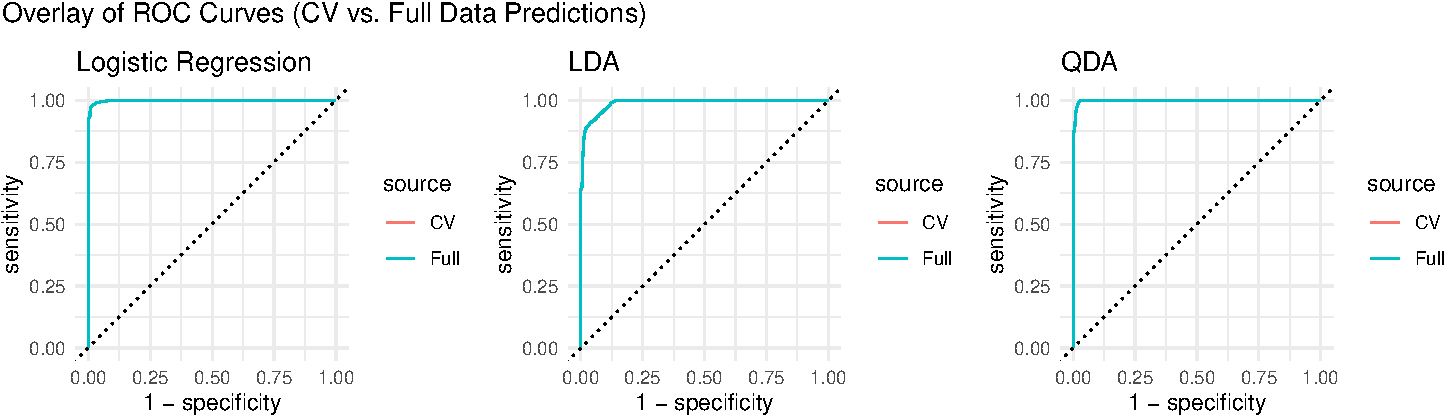
\includegraphics{ProjectPart1_MERGED_files/figure-latex/unnamed-chunk-11-1} 

}

\caption{ROC curve comarison between corss-valication and full data set predictions}\label{fig:unnamed-chunk-11}
\end{figure}

As we can see that the ROC curve for the cross-validation predictions is
almost identical to the ROC curve for the predictions on the full
training set, indicating that the logistic regression model is not
overfitting the training data.

\begin{Shaded}
\begin{Highlighting}[]
\CommentTok{\# Find optimal thresholds}
\NormalTok{threshold\_scan }\OtherTok{\textless{}{-}} \ControlFlowTok{function}\NormalTok{(model, data, model\_name) \{}
\NormalTok{  threshold\_data }\OtherTok{\textless{}{-}}\NormalTok{ model }\SpecialCharTok{\%\textgreater{}\%}
    \FunctionTok{augment}\NormalTok{(data) }\SpecialCharTok{\%\textgreater{}\%}
\NormalTok{    probably}\SpecialCharTok{::}\FunctionTok{threshold\_perf}\NormalTok{(}
      \AttributeTok{truth =}\NormalTok{ BT,}
      \AttributeTok{estimate =}\NormalTok{ .pred\_TRUE,}
      \AttributeTok{thresholds =} \FunctionTok{seq}\NormalTok{(}\FloatTok{0.01}\NormalTok{, }\FloatTok{0.99}\NormalTok{, }\FloatTok{0.01}\NormalTok{),}
      \AttributeTok{event\_level =} \StringTok{"first"}\NormalTok{,}
      \AttributeTok{metrics =} \FunctionTok{metric\_set}\NormalTok{(f\_meas)}
\NormalTok{    )}
\NormalTok{  opt\_threshold }\OtherTok{\textless{}{-}}\NormalTok{ threshold\_data }\SpecialCharTok{\%\textgreater{}\%}
    \FunctionTok{drop\_na}\NormalTok{() }\SpecialCharTok{\%\textgreater{}\%}
    \FunctionTok{arrange}\NormalTok{(}\FunctionTok{desc}\NormalTok{(.estimate)) }\SpecialCharTok{\%\textgreater{}\%}
    \FunctionTok{slice}\NormalTok{(}\DecValTok{1}\NormalTok{)}
  \FunctionTok{list}\NormalTok{(}
    \AttributeTok{threshold =}\NormalTok{ opt\_threshold}\SpecialCharTok{$}\NormalTok{.threshold,}
    \AttributeTok{threshold\_data =}\NormalTok{ threshold\_data,}
    \AttributeTok{opt\_threshold =}\NormalTok{ opt\_threshold,}
    \AttributeTok{model\_name =}\NormalTok{ model\_name}
\NormalTok{  )}
\NormalTok{\}}
\end{Highlighting}
\end{Shaded}

\begin{Shaded}
\begin{Highlighting}[]
\CommentTok{\# Fitted models}
\NormalTok{logreg\_result }\OtherTok{\textless{}{-}} \FunctionTok{threshold\_scan}\NormalTok{(final\_logreg\_fit, holdout\_data, }\StringTok{"Logistic Regression"}\NormalTok{)}
\NormalTok{lda\_result    }\OtherTok{\textless{}{-}} \FunctionTok{threshold\_scan}\NormalTok{(final\_lda\_fit, holdout\_data, }\StringTok{"LDA"}\NormalTok{)}
\NormalTok{qda\_result    }\OtherTok{\textless{}{-}} \FunctionTok{threshold\_scan}\NormalTok{(final\_qda\_fit, holdout\_data, }\StringTok{"QDA"}\NormalTok{)}
\end{Highlighting}
\end{Shaded}

\begin{Shaded}
\begin{Highlighting}[]
\CommentTok{\# Optimal thresholds}
\NormalTok{logreg\_holdout\_threshold }\OtherTok{\textless{}{-}}\NormalTok{ logreg\_result}\SpecialCharTok{$}\NormalTok{threshold}
\NormalTok{lda\_holdout\_threshold    }\OtherTok{\textless{}{-}}\NormalTok{ lda\_result}\SpecialCharTok{$}\NormalTok{threshold}
\NormalTok{qda\_holdout\_threshold    }\OtherTok{\textless{}{-}}\NormalTok{ qda\_result}\SpecialCharTok{$}\NormalTok{threshold}
\end{Highlighting}
\end{Shaded}

\begin{Shaded}
\begin{Highlighting}[]
\NormalTok{threshold\_scan\_cv }\OtherTok{\textless{}{-}} \ControlFlowTok{function}\NormalTok{(cv\_obj, model\_name) \{}
\NormalTok{  threshold\_data }\OtherTok{\textless{}{-}}\NormalTok{ cv\_obj }\SpecialCharTok{\%\textgreater{}\%}
    \FunctionTok{collect\_predictions}\NormalTok{() }\SpecialCharTok{\%\textgreater{}\%}
\NormalTok{    probably}\SpecialCharTok{::}\FunctionTok{threshold\_perf}\NormalTok{(}
      \AttributeTok{truth =}\NormalTok{ BT,}
      \AttributeTok{estimate =}\NormalTok{ .pred\_TRUE,}
      \AttributeTok{thresholds =} \FunctionTok{seq}\NormalTok{(}\FloatTok{0.05}\NormalTok{, }\FloatTok{0.95}\NormalTok{, }\FloatTok{0.01}\NormalTok{),}
      \AttributeTok{event\_level =} \StringTok{"first"}\NormalTok{,}
      \AttributeTok{metrics =} \FunctionTok{metric\_set}\NormalTok{(f\_meas)}
\NormalTok{    )}
\NormalTok{  opt\_threshold }\OtherTok{\textless{}{-}}\NormalTok{ threshold\_data }\SpecialCharTok{\%\textgreater{}\%}
    \FunctionTok{drop\_na}\NormalTok{() }\SpecialCharTok{\%\textgreater{}\%}
    \FunctionTok{arrange}\NormalTok{(}\FunctionTok{desc}\NormalTok{(.estimate)) }\SpecialCharTok{\%\textgreater{}\%}
    \FunctionTok{slice}\NormalTok{(}\DecValTok{1}\NormalTok{)}
  \FunctionTok{list}\NormalTok{(}
    \AttributeTok{threshold =}\NormalTok{ opt\_threshold}\SpecialCharTok{$}\NormalTok{.threshold}
\NormalTok{  )}
\NormalTok{\}}

\CommentTok{\# CV objects}
\NormalTok{logreg\_train\_result }\OtherTok{\textless{}{-}} \FunctionTok{threshold\_scan\_cv}\NormalTok{(logreg\_cv, }\StringTok{"Logistic Regression"}\NormalTok{)}
\NormalTok{lda\_train\_result    }\OtherTok{\textless{}{-}} \FunctionTok{threshold\_scan\_cv}\NormalTok{(lda\_cv, }\StringTok{"LDA"}\NormalTok{)}
\NormalTok{qda\_train\_result    }\OtherTok{\textless{}{-}} \FunctionTok{threshold\_scan\_cv}\NormalTok{(qda\_cv, }\StringTok{"QDA"}\NormalTok{)}

\CommentTok{\# Optimal thresholds}
\NormalTok{logreg\_train\_threshold }\OtherTok{\textless{}{-}}\NormalTok{ logreg\_train\_result}\SpecialCharTok{$}\NormalTok{threshold}
\NormalTok{lda\_train\_threshold    }\OtherTok{\textless{}{-}}\NormalTok{ lda\_train\_result}\SpecialCharTok{$}\NormalTok{threshold}
\NormalTok{qda\_train\_threshold    }\OtherTok{\textless{}{-}}\NormalTok{ qda\_train\_result}\SpecialCharTok{$}\NormalTok{threshold}
\end{Highlighting}
\end{Shaded}

\begin{Shaded}
\begin{Highlighting}[]
\CommentTok{\# Plot and combine threshold graphs}
\NormalTok{plot\_threshold }\OtherTok{\textless{}{-}} \ControlFlowTok{function}\NormalTok{(result) \{}
  \FunctionTok{ggplot}\NormalTok{(result}\SpecialCharTok{$}\NormalTok{threshold\_data, }\FunctionTok{aes}\NormalTok{(}\AttributeTok{x =}\NormalTok{ .threshold, }\AttributeTok{y =}\NormalTok{ .estimate)) }\SpecialCharTok{+}
    \FunctionTok{geom\_line}\NormalTok{() }\SpecialCharTok{+}
    \FunctionTok{geom\_point}\NormalTok{(}\AttributeTok{data =}\NormalTok{ result}\SpecialCharTok{$}\NormalTok{opt\_threshold, }\AttributeTok{color =} \StringTok{"red"}\NormalTok{, }\AttributeTok{size =} \DecValTok{2}\NormalTok{) }\SpecialCharTok{+}
    \FunctionTok{labs}\NormalTok{(}\AttributeTok{title =}\NormalTok{ result}\SpecialCharTok{$}\NormalTok{model\_name, }\AttributeTok{x =} \StringTok{"Threshold"}\NormalTok{, }\AttributeTok{y =} \StringTok{"F{-}Measure"}\NormalTok{) }\SpecialCharTok{+}
    \FunctionTok{coord\_cartesian}\NormalTok{(}\AttributeTok{ylim =} \FunctionTok{c}\NormalTok{(}\DecValTok{0}\NormalTok{, }\DecValTok{1}\NormalTok{))}
\NormalTok{\}}

\NormalTok{g1 }\OtherTok{\textless{}{-}} \FunctionTok{plot\_threshold}\NormalTok{(logreg\_result)}
\NormalTok{g2 }\OtherTok{\textless{}{-}} \FunctionTok{plot\_threshold}\NormalTok{(lda\_result)}
\NormalTok{g3 }\OtherTok{\textless{}{-}} \FunctionTok{plot\_threshold}\NormalTok{(qda\_result)}

\CommentTok{\# Combine the plots}
\NormalTok{g1 }\SpecialCharTok{+}\NormalTok{ g2 }\SpecialCharTok{+}\NormalTok{ g3}
\end{Highlighting}
\end{Shaded}

\begin{center}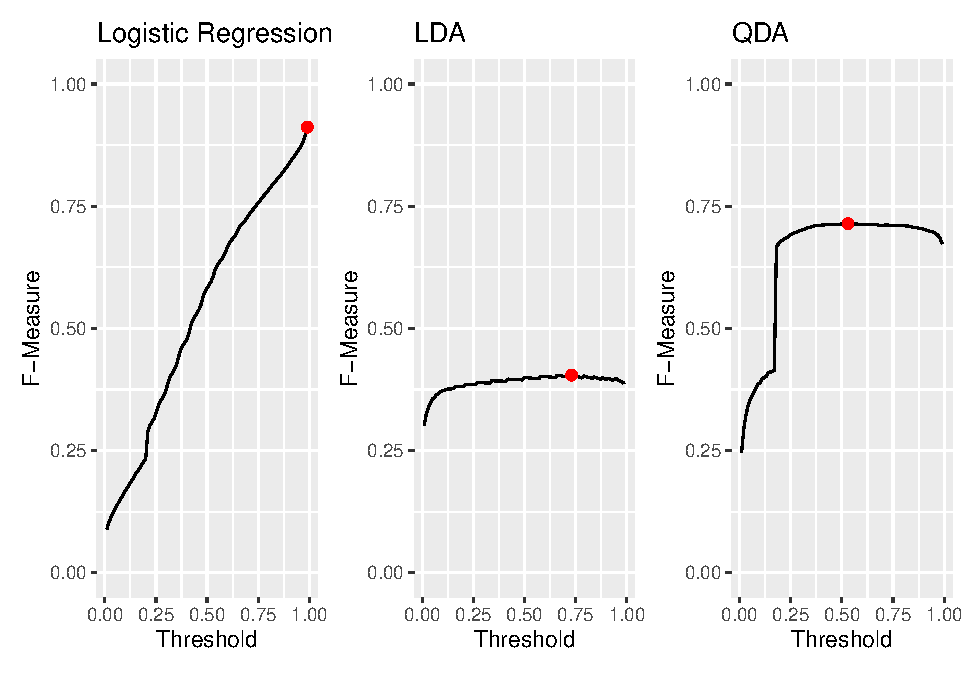
\includegraphics{ProjectPart1_MERGED_files/figure-latex/combine threshold graphs-1} \end{center}

\begin{Shaded}
\begin{Highlighting}[]
\NormalTok{predict\_at\_threshold }\OtherTok{\textless{}{-}} \ControlFlowTok{function}\NormalTok{(model, data, threshold) \{}
\NormalTok{  model }\SpecialCharTok{\%\textgreater{}\%}
    \FunctionTok{augment}\NormalTok{(data) }\SpecialCharTok{\%\textgreater{}\%}
    \FunctionTok{mutate}\NormalTok{(}\AttributeTok{.pred\_class =} \FunctionTok{make\_two\_class\_pred}\NormalTok{(.pred\_TRUE,}
                     \FunctionTok{c}\NormalTok{(}\StringTok{"TRUE"}\NormalTok{, }\StringTok{"FALSE"}\NormalTok{),}
                     \AttributeTok{threshold =}\NormalTok{ threshold))}
\NormalTok{\}}

\NormalTok{calculate\_metrics\_at\_threshold }\OtherTok{\textless{}{-}} \ControlFlowTok{function}\NormalTok{(model, train, holdout, model\_name, train\_threshold, holdout\_threshold) \{}
  \FunctionTok{bind\_rows}\NormalTok{(}
    \CommentTok{\# Metrics for the training set}
    \FunctionTok{bind\_cols}\NormalTok{(}
      \AttributeTok{model =}\NormalTok{ model\_name,}
      \AttributeTok{dataset =} \StringTok{"train"}\NormalTok{,}
      \AttributeTok{threshold =}\NormalTok{ train\_threshold,}
      \FunctionTok{metrics}\NormalTok{(}\FunctionTok{predict\_at\_threshold}\NormalTok{(model, train, train\_threshold), }\AttributeTok{truth =}\NormalTok{ BT, }\AttributeTok{estimate =}\NormalTok{ .pred\_class)}
\NormalTok{    ),}
    \FunctionTok{bind\_cols}\NormalTok{(}
      \AttributeTok{model =}\NormalTok{ model\_name,}
      \AttributeTok{dataset =} \StringTok{"train"}\NormalTok{,}
      \AttributeTok{threshold =}\NormalTok{ train\_threshold,}
      \FunctionTok{roc\_auc}\NormalTok{(model }\SpecialCharTok{\%\textgreater{}\%} \FunctionTok{augment}\NormalTok{(train), BT, .pred\_TRUE, }\AttributeTok{event\_level =} \StringTok{"first"}\NormalTok{)}
\NormalTok{    ),}
    \FunctionTok{bind\_cols}\NormalTok{(}
      \AttributeTok{model =}\NormalTok{ model\_name,}
      \AttributeTok{dataset =} \StringTok{"train"}\NormalTok{,}
      \AttributeTok{threshold =}\NormalTok{ train\_threshold,}
      \FunctionTok{f\_meas}\NormalTok{(}\FunctionTok{predict\_at\_threshold}\NormalTok{(model, train, train\_threshold), }\AttributeTok{truth =}\NormalTok{ BT, }\AttributeTok{estimate =}\NormalTok{ .pred\_class)}
\NormalTok{    ),}
    \FunctionTok{bind\_cols}\NormalTok{(}
      \AttributeTok{model =}\NormalTok{ model\_name,}
      \AttributeTok{dataset =} \StringTok{"train"}\NormalTok{,}
      \AttributeTok{threshold =}\NormalTok{ train\_threshold,}
      \FunctionTok{sens}\NormalTok{(}\FunctionTok{predict\_at\_threshold}\NormalTok{(model, train, train\_threshold), }\AttributeTok{truth =}\NormalTok{ BT, }\AttributeTok{estimate =}\NormalTok{ .pred\_class)}
\NormalTok{    ),}
    \CommentTok{\# Metrics for the holdout set}
    \FunctionTok{bind\_cols}\NormalTok{(}
      \AttributeTok{model =}\NormalTok{ model\_name,}
      \AttributeTok{dataset =} \StringTok{"holdout"}\NormalTok{,}
      \AttributeTok{threshold =}\NormalTok{ holdout\_threshold,}
      \FunctionTok{metrics}\NormalTok{(}\FunctionTok{predict\_at\_threshold}\NormalTok{(model, holdout, holdout\_threshold), }\AttributeTok{truth =}\NormalTok{ BT, }\AttributeTok{estimate =}\NormalTok{ .pred\_class)}
\NormalTok{    ),}
    \FunctionTok{bind\_cols}\NormalTok{(}
      \AttributeTok{model =}\NormalTok{ model\_name,}
      \AttributeTok{dataset =} \StringTok{"holdout"}\NormalTok{,}
      \AttributeTok{threshold =}\NormalTok{ holdout\_threshold,}
      \FunctionTok{roc\_auc}\NormalTok{(model }\SpecialCharTok{\%\textgreater{}\%} \FunctionTok{augment}\NormalTok{(holdout), BT, .pred\_TRUE, }\AttributeTok{event\_level =} \StringTok{"first"}\NormalTok{)}
\NormalTok{    ),}
    \FunctionTok{bind\_cols}\NormalTok{(}
      \AttributeTok{model =}\NormalTok{ model\_name,}
      \AttributeTok{dataset =} \StringTok{"holdout"}\NormalTok{,}
      \AttributeTok{threshold =}\NormalTok{ holdout\_threshold,}
      \FunctionTok{f\_meas}\NormalTok{(}\FunctionTok{predict\_at\_threshold}\NormalTok{(model, holdout, holdout\_threshold), }\AttributeTok{truth =}\NormalTok{ BT, }\AttributeTok{estimate =}\NormalTok{ .pred\_class)}
\NormalTok{    ),}
    \FunctionTok{bind\_cols}\NormalTok{(}
      \AttributeTok{model =}\NormalTok{ model\_name,}
      \AttributeTok{dataset =} \StringTok{"holdout"}\NormalTok{,}
      \AttributeTok{threshold =}\NormalTok{ holdout\_threshold,}
      \FunctionTok{sens}\NormalTok{(}\FunctionTok{predict\_at\_threshold}\NormalTok{(model, holdout, holdout\_threshold), }\AttributeTok{truth =}\NormalTok{ BT, }\AttributeTok{estimate =}\NormalTok{ .pred\_class)}
\NormalTok{    )}
\NormalTok{  )}
\NormalTok{\}}

\NormalTok{metrics\_at\_threshold }\OtherTok{\textless{}{-}} \FunctionTok{bind\_rows}\NormalTok{(}
    \FunctionTok{calculate\_metrics\_at\_threshold}\NormalTok{(final\_logreg\_fit, train\_data, holdout\_data, }\StringTok{"Logistic regression"}\NormalTok{, logreg\_train\_threshold, logreg\_holdout\_threshold),}
    \FunctionTok{calculate\_metrics\_at\_threshold}\NormalTok{(final\_lda\_fit, train\_data, holdout\_data, }\StringTok{"LDA"}\NormalTok{, lda\_train\_threshold, lda\_holdout\_threshold),}
    \FunctionTok{calculate\_metrics\_at\_threshold}\NormalTok{(final\_qda\_fit, train\_data, holdout\_data, }\StringTok{"QDA"}\NormalTok{, qda\_train\_threshold, qda\_holdout\_threshold)}
\NormalTok{) }\SpecialCharTok{\%\textgreater{}\%} \FunctionTok{arrange}\NormalTok{(dataset)}
\end{Highlighting}
\end{Shaded}

\begin{Shaded}
\begin{Highlighting}[]
\NormalTok{metrics\_at\_threshold }\SpecialCharTok{\%\textgreater{}\%}
        \FunctionTok{pivot\_wider}\NormalTok{(}\AttributeTok{names\_from=}\NormalTok{.metric, }\AttributeTok{values\_from=}\NormalTok{.estimate) }\SpecialCharTok{\%\textgreater{}\%}
        \FunctionTok{select}\NormalTok{(}\SpecialCharTok{{-}}\NormalTok{.estimator) }\SpecialCharTok{\%\textgreater{}\%}
\NormalTok{        knitr}\SpecialCharTok{::}\FunctionTok{kable}\NormalTok{(}
          \AttributeTok{caption=} \StringTok{"Performance metrics for models at ideal threshold."}\NormalTok{, }
          \AttributeTok{digits=}\DecValTok{3}\NormalTok{) }\SpecialCharTok{\%\textgreater{}\%}
\NormalTok{        kableExtra}\SpecialCharTok{::}\FunctionTok{kable\_styling}\NormalTok{(}\AttributeTok{full\_width=}\ConstantTok{FALSE}\NormalTok{)}
\end{Highlighting}
\end{Shaded}

\begin{longtable}[t]{llrrrrrr}
\caption{\label{tab:model eval table}Performance metrics for models at ideal threshold.}\\
\toprule
model & dataset & threshold & accuracy & kap & roc\_auc & f\_meas & sens\\
\midrule
Logistic regression & holdout & 0.99 & 0.999 & 0.911 & 0.999 & 0.912 & 0.953\\
LDA & holdout & 0.73 & 0.983 & 0.398 & 0.992 & 0.404 & 0.797\\
QDA & holdout & 0.53 & 0.996 & 0.712 & 0.992 & 0.714 & 0.689\\
Logistic regression & train & 0.21 & 0.996 & 0.932 & 0.999 & 0.934 & 0.926\\
LDA & train & 0.84 & 0.985 & 0.755 & 0.989 & 0.763 & 0.759\\
\addlinespace
QDA & train & 0.23 & 0.995 & 0.911 & 0.998 & 0.914 & 0.866\\
\bottomrule
\end{longtable}

\begin{Shaded}
\begin{Highlighting}[]
\NormalTok{visualize\_conf\_mat\_holdout }\OtherTok{\textless{}{-}} \ControlFlowTok{function}\NormalTok{(model, data, threshold, metric\_label) \{}
\NormalTok{  cm }\OtherTok{\textless{}{-}}\NormalTok{ model }\SpecialCharTok{\%\textgreater{}\%}
    \FunctionTok{augment}\NormalTok{(data) }\SpecialCharTok{\%\textgreater{}\%}
    \FunctionTok{mutate}\NormalTok{(}\AttributeTok{.pred\_class =} \FunctionTok{make\_two\_class\_pred}\NormalTok{(.pred\_TRUE, }\FunctionTok{c}\NormalTok{(}\StringTok{"TRUE"}\NormalTok{, }\StringTok{"FALSE"}\NormalTok{), }\AttributeTok{threshold =}\NormalTok{ threshold)) }\SpecialCharTok{\%\textgreater{}\%}
    \FunctionTok{conf\_mat}\NormalTok{(}\AttributeTok{truth =}\NormalTok{ BT, }\AttributeTok{estimate =}\NormalTok{ .pred\_class)}
  
  \FunctionTok{autoplot}\NormalTok{(cm, }\AttributeTok{type =} \StringTok{"heatmap"}\NormalTok{) }\SpecialCharTok{+}
    \FunctionTok{labs}\NormalTok{(}\AttributeTok{title =} \FunctionTok{sprintf}\NormalTok{(}\StringTok{"Threshold \%.2f (\%s)"}\NormalTok{, threshold, metric\_label))}
\NormalTok{\}}

\NormalTok{overview\_model\_holdout }\OtherTok{\textless{}{-}} \ControlFlowTok{function}\NormalTok{(model, model\_name, threshold) \{}
\NormalTok{  cm\_plot }\OtherTok{\textless{}{-}} \FunctionTok{visualize\_conf\_mat\_holdout}\NormalTok{(model, holdout\_data, threshold, }\StringTok{"Holdout"}\NormalTok{)}
\NormalTok{  cm\_plot }\SpecialCharTok{+} \FunctionTok{labs}\NormalTok{(}\AttributeTok{title =} \FunctionTok{sprintf}\NormalTok{(}\StringTok{"\%s }\SpecialCharTok{\textbackslash{}n}\StringTok{ (Threshold = \%.2f)"}\NormalTok{, model\_name, threshold))}
\NormalTok{\}}

\NormalTok{logreg\_cm }\OtherTok{\textless{}{-}} \FunctionTok{overview\_model\_holdout}\NormalTok{(final\_logreg\_fit, }\StringTok{"Logistic Regression"}\NormalTok{, logreg\_holdout\_threshold)}
\NormalTok{lda\_cm    }\OtherTok{\textless{}{-}} \FunctionTok{overview\_model\_holdout}\NormalTok{(final\_lda\_fit, }\StringTok{"LDA"}\NormalTok{, lda\_holdout\_threshold)}
\NormalTok{qda\_cm    }\OtherTok{\textless{}{-}} \FunctionTok{overview\_model\_holdout}\NormalTok{(final\_qda\_fit, }\StringTok{"QDA"}\NormalTok{, qda\_holdout\_threshold)}
\end{Highlighting}
\end{Shaded}

\begin{Shaded}
\begin{Highlighting}[]
\NormalTok{logreg\_cm }\SpecialCharTok{+}\NormalTok{ lda\_cm }\SpecialCharTok{+}\NormalTok{ qda\_cm}
\end{Highlighting}
\end{Shaded}

\begin{figure}[H]

{\centering 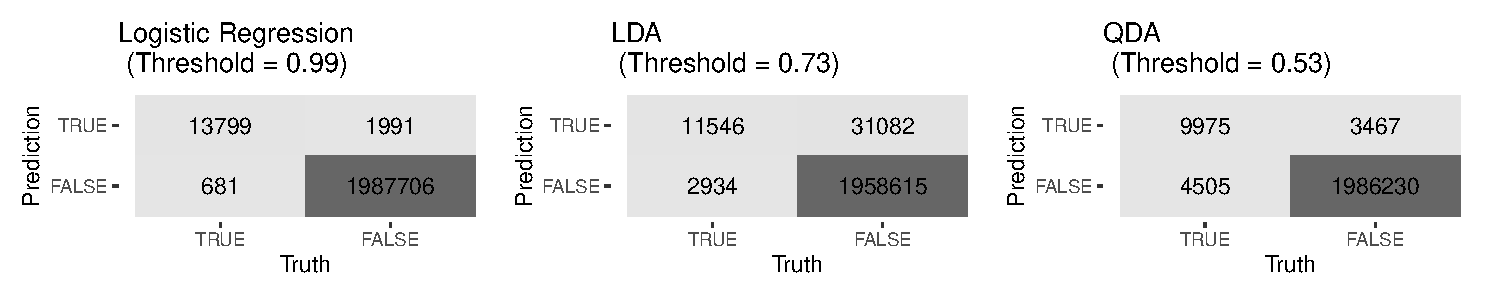
\includegraphics{ProjectPart1_MERGED_files/figure-latex/unnamed-chunk-16-1} 

}

\caption{ROC curve comarison between corss-valication and full data set predictions}\label{fig:unnamed-chunk-16}
\end{figure}

\begin{Shaded}
\begin{Highlighting}[]
\FunctionTok{stopCluster}\NormalTok{(cl)}
\FunctionTok{registerDoSEQ}\NormalTok{()}
\end{Highlighting}
\end{Shaded}


\end{document}
